\chapter{Úvod}

Svět webových technologií se neustále vyvíjí, rok za rokem stoupá výkon klientských zařízení a spolu s
ním i velikost a komplexita webových aplikací. Co se ale bohužel zlepšuje jen velmi pozvolna, je rychlost
webových aplikací. Problém nízké rychlosti se navíc postupně zvětšuje, kvůli zvyšujícímu se zastoupení
uživatelů, kteří pro přístup k webovým aplikacím používají mobilní zařízení s malým výkonem a nepříliš
dobrou konektivitou.

V posledních letech se stále častěji můžeme setkat s webovými stránkami, které používají open source technologii \emph{Accelerated Mobile Pages} neboli zkráceně \emph{AMP}, která se snaží problém rychlosti webových aplikací
řešit pomocí omezení složitosti, optimalizací vykreslování (díky fixnímu rozložení), přednačítání webové
stránky a dalších optimalizací v rámci \emph{AMP distribuční infrastruktury}.

Výsledkem všech těchto optimalizací jsou webové stránky, jejichž čas do první interakce\footnote{Čas do první interakce: anglicky se tato metrika nazývá Time to Interactive a vyjadřuje, jak dlouho trvá, než se stránka načte do stavu, kdy je uživatel schopný s ní bez omezení interagovat.} je v nízkých desetinách sekundy. Pro porovnání v roce 2018 průměrně trvalo načtení webové
stránky 8.66s\cite{TTI}.
Udržení rychlosti načítání stránky na takto nízkých hranicích ovlivňuje, jak se uživatel po příchodu na naši
stránku bude chovat (a zda si nerozmyslí, naši stránku vůbec nenavštívit).

Zvýšená rychlost \emph{AMP} stránek má kromě přímých efektů na uživatele také vedlejší efekt na pozici
v rámci výsledků vyhledávání a tím i na větší počet návštěvníků.

Jako každá jiná technologie tak i \emph{AMP} technologie není všemocná a pro její použití musí vývojáři
obětovat většinu interaktivity pomocí \emph{javascriptu}, značně omezit velikost kaskádových stylů a zcela
vynechat některé zakázané \emph{HTML} tagy. Kvůli těmto omezením jsou cílovými použitími pro \emph{AMP} jednoduché statické stránky, popřípadě značně
zjednodušené verze stránek plnohodnotných.

Cílem této práce je přinést výše zmiňované výhody technologie \emph{AMP} uživatelům open source webového
frameworku \emph{DotVVM} založeného na platformě \emph{ASP.NET}.
Přestože cílovým použitím \emph{DotVVM} jsou složité interaktivní webové aplikace (tedy opak stránek ideálních pro přepis do \emph{AMP}), tak i v rámci těchto aplikací často nalezneme stránky, které jsou z velké části statické, popřípadě se dynamicky skládají na serveru, ale ne už u klienta \cite{DotVVMIntro}. Příkladem takových stránek můžou být úvodní a další veřejné/informační stránky u jinak dynamických webových aplikací. 

\chapter{Co to je AMP?}
\label{AMP}
Technologie \emph{AMP} má za cíl zajistit uživatelům velmi rychlé webové stránky nezávisle na tom, kde se
uživatelé nacházejí a jaké zařízení používají.

\emph{AMP} byl původně vydán v roce 2015 společností Google (ve spolupráci s firmou Twitter) pod názvem \emph{Accelerated Mobile Pages} jako odpověď
na technologii Facebooku s názvem \emph{Instant Articles}. Na rozdíl od \emph{Instant Articles} se \emph{AMP}, díky tomu že je
open-source, rozšířil mimo platformu zakládající organizace a nyní existují více než dvě miliardy AMP
stránek~\cite{AMPTurbo}.

Amp zajištuje slibované zvýšení rychlosti pomocí kombinace dvou přístupů. Redukce komplexity webových stránek, která je vynucovaná mnohými restrikcemi technologie AMP, a přiblížení obsahu uživatelům pomocí distribuovaných AMP Cache a dalších souřástí AMP infrastruktury. Kromě společnosti Google dnes poskytují kompletní infrastrukturu pro AMP stránky také
společnosti Microsoft a~CloudFlare.

\section{Nové typy obsahu, které AMP přináší}
Kromě celých webových stránek \emph{AMP} podporuje i další nové typy obsahu. Tyto nové formáty přináší novou funkcionalitu a zvýšení rychlosti do domén jako je například email nebo reklama. Žádný z těchto nových formátů se bohužel prozatím nerozšířil mimo Google platformu. Uživatelé se nejčastěji mohou setkat s AMP adds, ale to jen z toho důvodu že \emph{Google AdSense}\footnote{Google AdSence je platforma společnosti Google, která umožnuje si zakoupit reklamní prostor na různých webových stránkách.} je hlavní provozovatel reklamních služeb na internetu.
\subsection*{AMP Email}
\emph{Amp Email} umožňuje používat v rámci emailů \emph{AMP} komponenty. Díky tomu mohou emaily obsahovat formuláře, interaktivní grafiku a další prvky, které byly dosud vyhrazené jen pro web. \emph{AMP Email} má formát \emph{HTML} s atributem amp4email. V rámci jednoho \emph{AMP} emailu by měla být vždy posílána i textová a případně webová verze, jinak by nastával problém při starších emailových klientech\cite[Ch.\ 6, p.\ 285]{VzhuruDoAMP}.
Aktuálně je \emph{AMP Email} podporován jen v klientech:
Outlook, Gmail a Mail.ru\cite{EmailSupport}.
\subsection*{AMP Add}
Reklamy bez \emph{javascriptu} fungovat skoro nemohou. A přestože pro koncové uživatele by byl web bez reklam ideální, tak z pohledu některých provozovatelů by bylo toto omezení likvidační. \emph{AMP} tento problém řeší pomocí \emph{AMP} komponenty \emph{AMP Add}, které umožnuje vložit do stránky reklamní bannery. Díky tomu, že \emph{AMP} přesně ví které prvky na stránce jsou reklama, tak může zařídit, aby se na tyto pro uživatele nedůležité prvky nečekalo. Stránky, které budou zobrazovány v rámci \emph{AMP Add} musí být vydány schváleným provozovatelem a \emph{HTML} reklamního banneru musí být anotováno atributem \emph{amp4add}\cite[Ch.\ 6, p.\ 280]{VzhuruDoAMP}.
V lednu 2019 tvořili \emph{AMP} reklamy 12\% všech reklamy v rámci \emph{Google AdSense}\cite{abner_2019}.
\subsection*{AMP Stories}
AMP Stories jsou celoobrazovkové “prezentace” vizuálně velmi podobné konceptu stories od společnosti Facebook. Tento typ obsahu je určen především pro zpravodajské portály, které jej mohou využít pro vytvoření krátkých
“prezentací” k danému tématu. Na tyto prezentace poté uživatelé mohou přistoupit po hledání jména
vydavatele v rámci prohlížeče nebo při hledání k samotné události, kterou \emph{AMP story} popisuje\cite[Ch.\ 6, p.\ 290]{VzhuruDoAMP}.

\section{Základní principy technologie AMP}
Technologie \emph{AMP} se skládá ze dvou hlavních částí: \emph{AMP frameworku} a \emph{AMP distribuční infrastruktury}. 

\begin{table}[H]
	\caption{Tabulka jednotlivých součástí technologie AMP} 
	\centering
	\begin{tabular}{m{15em} | m{15em}}
		\toprule
		\cmidrule(r){1-2}
		FRAMEWORK & DISTRIBUCE \\
		\midrule
		AMP HTML & AMP Cache \\
		AMP CSS & AMP Viewer \\
		AMP Komponenty & AMP Prerender \\
		\bottomrule
	\end{tabular}
	\label{tab:Součásti technologie AMP}
\end{table}

Jednotlivé komponenty \emph{AMP frameworku} slouží pro sestavení samotné \emph{AMP} stránky. Na rozdíl od svých
ne-AMP ekvivalentů jsou ořezané o některé funkce, při jejichž použití mohou být stránky pomalé a/nebo
by docházelo k dynamickým změnám rozložení. Pokud by docházelo k dynamickým změnám rozložení,
tak by nebylo možné provádět prerendering.


Prvky distribučního procesu se různými metodami snaží minimalizovat čas potřebný k zobrazení stránky
uživateli. Distribuční \emph{AMP} infrastrukturu provozují aktuálně Google, Microsoft a CloudFlare\cite[Ch.\ 1, p.\ 49]{VzhuruDoAMP}.

\subsection*{AMP Framework}
\emph{AMP} stránky jsou tvořeny ve zjednodušeném jazyku \emph{HTML}, který je rozšířený o \emph{AMP} atributy a \emph{AMP}
komponenty. Omezení se nevyhnulo ani kaskádovým stylům. Jejich velikost je omezena na pouhých
75\,kB, musí být umístěny přímo v dokumentu a nelze použít všechny typy animací a některé další
konstrukty CSS.
Největší omezení \emph{AMP} technologie ale rozhodně představuje absence skoro jakéhokoliv \emph{javascriptu}.
Kvůli těmto omezením mají \emph{AMP} stránky statický layout. Statický layout umožnuje, aby byla \emph{AMP} stránka před vykreslená návštěvníkovi dříve než se vůbec rozhodne, že na danou stránku chce přistoupit. \emph{AMP Prerendering} je hlavní důvod, proč je \emph{AMP} schopen zobrazit před stránky v čase blížícím se nule\cite{AMP-zero}.
\subsubsection*{AMP Html}
\emph{AMP Html} vychází z \emph{HTML 5}, je ale značně upravené. Některé základní \emph{HTML} tagy jsou nahrazeny jejich \emph{AMP} variantami a některé jsou zakázány.
Oproti klasickému \emph{HTML} můžeme \emph{AMP Html} rozeznat podle bezhodnotového atributu s názvem amp (případně emotikonu High Voltage).

\begin{lstlisting}[language=html, caption=Ukázka AMP Html,captionpos=t]
<!doctype html>
<html amp lang="cs">
<head>
    <meta charset="utf-8">
    <meta name="viewport" content="width=device-width,minimum-scale=1">
    <script async src="https://cdn.ampproject.org/v0.js"></script>
    <style amp-custom>
        /*INLINE CSS*/
    </style>
    <style amp-boilerplate>
        /* AMP BOILER PLATE CSS */
    </style>
    <link rel="canonical" href="UmisteniPuvodniStranky">
    <title>AMP</title>
</head>
<body>
    <h1>Toto je AMP stranka</h1>
</body>
</html>

\end{lstlisting}

\smallHeading{Hlavička}
V rámci hlavičky \emph{AMP} dokumentu je nutné přidat \emph{AMP} knihovnu a amp-boilerplate css\footnote{Plné znění amp-boilerplate css je možné nalézt na \url{https://amp.dev/boilerplate/}}\cite{AMPBoilerplate}.

Toto css má za úkol skrýt stránku, dokud není plně vyrenderované a následně ji pomocí animace prolnutí zobrazit. Díky tomuto je stránka pocitově rychlejší.
Vynechání těchto dvou prvků by způsobilo nevalidnost \emph{AMP} stránky => amp stránka se nedostane do cache.

V rámci hlavičky také můžeme přidat odkaz na požadované fonty. V rámci \emph{AMP} stránek jsou povoleny jen fonty dostupné na zdrojích uvedených v tabulce \ref{tab:Tabulka povolených zdrojů fontů}\cite{ampCustomFonts}.

\begin{table}[H]
	\caption{Tabulka povolených poskytovatelů fontů}
	\centering
	\begin{tabular}{m{10em} | m{20em}}
		\toprule
		\cmidrule(r){1-2}
		TYPOGRAPHY.COM & \url{https://cloud.typography.com} \\ \midrule
		FONTS.COM & \url{https://fast.fonts.net} \\ \midrule
		GOOGLE FONTS & \url{https://fonts.googleapis.com} \\ \midrule
		TYPEKIT & \url{https://use.typekit.net} \\ \midrule
		FONT AWESOME & \url{https://maxcdn.bootstrapcdn.com} \newline \url{https://use.fontawesome.com} \\
		\bottomrule
	\end{tabular}
	\label{tab:Tabulka povolených zdrojů fontů}
\end{table}

\smallHeading{AMP Html elementy}
Kvůli požadavku na fixní layout není možné použít všechny \emph{HTML} elementy, některé jsou zakázané \ref{tab: Tabulka zakázaných HTML elementů}, některé byly nahrazeny jejich \emph{AMP} variantami \ref{tab: Tabulka nahrazených AMP elementů} a u jiných je omezena jejich funkcionalita \ref{tab: Tabulka HTML elementů s omezenou funkcionalitou} \cite[p.\ 41]{AMP-ENG-Book}.

\begin{table}[H]
	\caption{Tabulka zakázaných HTML elementů} 
	\centering
	\begin{tabular}{c|c|c|c|c|c|c|c}
		\toprule
		base & picture & frame & frameset & object & param & applet & embed \\
		\bottomrule
	\end{tabular}
	\label{tab: Tabulka zakázaných HTML elementů}
\end{table}

\begin{table}[H]
	\caption{Tabulka nahrazených HTML elementů} 
	\centering
	\begin{tabular}{m{15em}|m{15em}}
		\toprule
		img & amp-img \\ \midrule
		video & amp-video \\ \midrule
		audio & amp-audio \\ \midrule
		iframe & amp-iframe \\
		\bottomrule
	\end{tabular}
	\label{tab: Tabulka nahrazených AMP elementů}
\end{table}

\begin{table}[H]
	\caption{Tabulka HTML elementů s omezenou funkcionalitou}
	\centering
	\begin{tabular}{m{3em}|m{35em}}
		\toprule
		script & Povoleny jen typu \boldsymbol{application/ld+json} nebo \boldsymbol{text/plain}. \\ \midrule
		input & Typy: \boldsymbol{image}, \boldsymbol{button}, \boldsymbol{password} a  \boldsymbol{file} jsou zakázané.\\ \\ \midrule
		style & Povolen jen jediný styl v hlavičce (kromě \emp{amp-boilerplate}), tento styl musí mít atribut. \boldsymbol{amp-custom}. \\\\ \midrule
		a & Jsou zakázané javascriptové odkazy.\\
		\bottomrule
	\end{tabular}
	\label{tab: Tabulka HTML elementů s omezenou funkcionalitou}
\end{table}

\subsubsection*{AMP CSS}
V rámci \emph{AMP} stránky jsme omezeni pouze na max 75kB (dříve jen 50kB) inline \emph{CSS}\cite[Ch.\ 2 p.\ 100]{VzhuruDoAMP}. Důvodem, proč styly musí být přiloženy v rámci \emph{AMP} stránky, je snaha o minimalizaci počtu potřebných request k tomu, aby mohla být načtena stránka (nebo alespoň části ovlivňující její rozložení). Výjimkou jsou \emph{CSS keyframes}\footnote{CSS keyframes obsahují definice animací.}, které můžou být obsaženy v separátním inline \emph{CSS} elementu s maximální velikostí 500kB\cite{ampHTMLSpec}.

Kromě omezení velikosti a nutnosti styly přikládat k hlavnímu dokumentu, \emph{AMP} také zakazuje použití klíčového slova \emph{!important} a stylování \emph{AMP} komponent (selektory cílící na tagy začínající na \emph{-amp-} nebo \emph{i-amp-} )\cite{AMPCss}. Obě tato omezení jsou nutná kvůli tomu, aby~amp byl schopný zajistit, že elementy budou mít předpokládanou velikost.

Další omezení, se kterým musí vývojáři bojovat, je zákaz většiny animací. Jediné povolené animace jsou nad vlastnostmi, jejichž animovaní je \emph{GPU-accelerated}, jde tedy o animace nad vlastnostmi \emph{opacity} a \emph{transform}\cite{AMPCss}.

\subsubsection*{Omezení použití javascriptu}
Vlastní \emph{javascript} je aktuálně kompletně zakázaný v rámci stránky. Existuje však několik způsobů, jak \emph{javascript} spustit.
\smallHeading{iframe}
V rámci \emph{amp-iframe} můžeme používat jakýkoliv \emph{javascript}. Stejně jak u klasického \emph{HTML} \emph{iframe} tak i tady nemůžeme ovlivňovat nic mimo daný \emph{iframe}. Toto řešení se hodí, pokud potřebujeme například zobrazit mapy, apod.
\smallHeading{AMP-script}
Koncem roku 2019 byla vydaná komponenta \emph{AMP-script}. Tato dodatečná komponenta umožnuje spouštět \emph{javascript} v rámci \emph{Web Workeru}, tento kód běží na pozadí. V rámci tohoto kódu můžeme přidat interaktivitu do stránky například úpravami virtuálního \emph{DOMu} stránky nebo úpravou stavu komponenty \emph{amp-state}.

V rámci \emph{AMP-script} nejsou povoleny všechny \emph{javascriptové} API (podpora API pro manipulaci s prohlížečem chybí) a některé, jako například metoda \emph{querySelektor}, jsou omezené\cite{amp-script}.

\subsection*{Distribuční infrastruktura pro AMP stránky}

Přestože jsme schopni zobrazovat \emph{AMP} stránky bez využití distribučních mechanizmů \emph{AMPu}, tak jsme přišli o výhody přednačítání stránek a dalších optimalizací, za které jsou zodpovědné \emph{AMP Cache} a \emph{AMP Viewer}.
Bez těchto optimalizací je jediný benefit, který získáme použitím technologie \emph{AMP} ten, že nás tato technologie nutí tvořit jednoduché stránky a omezuje nás ve velikosti externě načítaných zdrojů. Část takto ušetřeného času bychom vzápětí zase ztratili kvůli nutností stažení \emph{AMP} knihovny.

\begin{figure}[hbt]
	\centering
	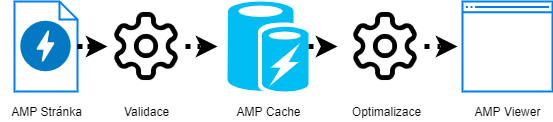
\includegraphics[width=1\textwidth]{obrazky-figures/AmpDistribuce.png}
	\caption{Popis distribuční infrastruktury}
	\label{Popis Distribuční infrastruktury AMP}
\end{figure}
\emph{Amp} distribuční infrastruktura se skládá ze dvou hlavních částí: \emph{AMP Cache} a \emph{AMP Vieweru}. Schéma této infrastruktury je znázorněno na obrázku \ref{Popis Distribuční infrastruktury AMP}.

\emph{Amp} stránka se do \emph{AMP cache} dostane jen tehdy, je-li validní a provozovatel \emph{AMP cache} usoudí, že se mu vyplatí danou stránku cachovat. Díky umístění stránky v \emph{AMP cache} získáme kromě přiblížení obsahu ke koncovým uživatelům také různé typy optimalizací.

Amp Viewer má na starosti prerendering stránek z \emph{AMP Cache}. Dalo by se říci, že je webovou aplikací obalující naší \emph{AMP stránku}. 

\subsubsection*{AMP Cache}
Základní funkcionalitou \emph{AMP cache} je poskytovat \emph{Content Delivery Network}\footnote{Content Delivery Network je služba, která umožnuje, aby se externí obsah stahoval ze serveru, který je blíže k cílovému uživateli.} pro \emph{AMP} stránky. Stránky uložené v \emph{AMP Cache} jsou poté přístupné pomocí \emph{AMP Vieweru}.
Kromě této základní funkcionality \emph{AMP Cache} také poskytuje mechanismy pro validaci a optimalizaci \emph{AMP} stránek.

\smallHeading{Validace}
Validace probíhá před samotným zařazením \emph{AMP} stránky do cache a její výsledek rozhoduje o tom, jestli bude do cache zařazena.
\emph{AMP} validace kontroluje, zda není porušeno některé z omezení a požadavků \emph{AMP frameworku}. Například zda stránka obsahuje jen validní elementy nebo zda obsahuje \emph{AMP} JS a CSS boiler plate.\cite{AMPCache}.

\smallHeading{Optimalizace}
Po zařazení \emph{AMP} stránky do cache probíhají dodatečné optimalizace obsahu.
Proběhne úprava \emph{HTML}, během které dojde k odstranění prázdných znaků a komentářů, a stránka se upraví tak, aby nebylo možné provést \emph{Cross-site scripting}\cite{whyAMPCache}.
Obrázky jsou zkomprimovány a jsou z nich odstraněna nepotřebná metadata. Pokud je to možné, dojde ke konverzi na \emph{WebP} formát a ke generaci \emph{srcsetů}.
Externí zdroje jsou anotovány prefetch značkami, toto umožní \emph{AMP Prerender}\footnote{Prerender: vykreslení stránky nebo její části ještě předtím, než si uživatel o obsah této stránky zažádá.}.
Nakonec dojde k agresivní minifikaci\footnote{Minifikace: odstranění nepotřebných prvků (mezery, komentáře,..) ze zdrojového kódu. Také může například docházet ke zkrácení názvů proměnných nebo funkcí.} \emph{HTML} a \emph{CSS}.

\smallHeading{Aktualizace}
Standardně \emph{AMP cache} provádí aktualizace uložených stránek dle principu \emph{stale-while-revalidate}, tzn. že pokud si uživatel vyžádá dokument, o kterém si\emph{AMP cache} myslí, že je neplatný (například  je překročená \emph{Max-Age} hlavička), tak mu \emph{AMP cache} předá tuto starou verzi a zažádá si o aktualizace, takže další uživatel dostane již verzi novou\cite{AMPUpdate}.
Majitel domény, v rámci které je \emph{AMP} stránka hostovaná, může také “manuálně“ zažádat o aktualizaci stránky pomocí \emph{update-cache} dotazu. Tento dotaz musí být podepsán privátním \emph{RSA} klíčem asociovaným s danou doménou\cite{AMPUpdateUrl}.

\subsubsection*{AMP Viewer}
\emp{AMP Viewer} je prostředí, ve kterém běží jednak kód hostované \emph{AMP} stránky, tak z části kód samotného \emph{AMP Vieweru}. Hlavní úlohou AMP Vieweru je optimalizaci zobrazení \emph{AMP} stránky a o její prerendering.

\smallHeading{AMP Prerendering}
Prerendering probíhá u \emph{AMP} stránek, o kterých si poskytovatel \emph{AMP Vieweru} myslí, že na ně budeme chtít přistoupit, ještě předtím, než na ně přistoupíme, tzn. že v jednu chvíli může být předpřipraveno více stránek. V jednu chvíli probíhá \emph{prerendering} jen pro jednu stránku. 
\begin{gatger}
\begin{enumerate}
    \item \emph{AMP Viewer} stáhne \emph{AMP HTML} z \emph{AMP Cache}
    \item Načte potřebné \emph{JS} knihovny
    \item Stáhne obrázky a další externí obsah vhodný pro dané zařízení. \\
    Dochází ke stažení jen toho obsahu, který se skutečně uživateli zobrazí okamžitě po příchodu na stránku\cite{ampConf}.
\end{enumerate}
\end{gatger}
\smallHeading{Nevýhody AMP Vieweru}
Z důvodu zobrazení naší \emph{AMP} stránky v rámci \emph{AMP Vieweru} dochází k tomu, že adresa, na které se uživatel nachází, nepřísluší naší stránce, ale je to adresa \emph{AMP Vieweru}. Toto \emph{AMP Viewer} aktuálně, pouze částečně, řeší pomocí falešného navigačního baru, který zobrazuje skutečnou zdrojovou adresu. Toto chování může zjednodušovat \emph{phishing} útoky\cite[Ch.\ 3, p.\ 50]{VzhuruDoAMP}.
Řešením tohoto problému je technologie \emph{Signed HTTP Exchange}, která umožní oddělit autora/zdroj obsahu od jeho poskytovatele\cite[Ch.\ 3, p.\ 51]{VzhuruDoAMP}.
\chapter{DotVVM}
\emph{DotVVM} je \emph{open source MVVM}\footnote{MVVM: návrhový vzor model - view - viewmodel.} webový framework\cite{DotVVMIntro}. \emph{Backend} část je založená na technologii \emph{ASP.NET} (případně na její \emph{.NET Core} variantě). Frontend je založený na značně upravené verzi \emph{javascriptové} knihovny \emph{Knockout}. Díky tomu, že \emph{DotVVM} pokrývá \emph{frontend} i \emph{backend}, jsme schopni psát relativně komplexní aplikace jen s použitím jazyka \emph{C\#} (popřípadě jiného jazyka z platformy \emph{.NET}) a jazyka \emph{DotHtml}\footnote{DotHtml: HTML rozšířené o nové tagy, vazby na ViewModel a předpisy vazby DotHtml na Viewmodel.}. Z velké části se tak vyhneme psaní javascriptu pro běžné a repetetivní úkony, jako například komunikace se serverem a mapování dat mezi formáty, které se používají na backendu a frontendu.
Díky těmto vlastnostem a snadné rozšiřitelnosti \emph{DotVVM} o vlastní komponenty a komponenty třetích stran, je programátor se znalostí platformy \emph{.NET} schopen velmi rychle vytvořit v~\emph{DotVVM} aplikaci.

\emph{DotVVM} je vhodný převážně pro tvorbu \emph{Line of Business} aplikací\footnote{Line of Business aplikace: Rozsáhlé informační systémy, které obsahují velké množství formulářů, tabulek, atd.}\cite{DotVVMIntro}. Pro čistě statické prezentační weby většinou nepřináší dostatek benefitů, které by vyvážily snížení rychlosti oproti stránkám používajícím kombinaci \emph{HTML} a jednoduchého \emph{javascriptu}. Ve chvílích, kdy ale potřebujeme mít v rámci \emph{DotVVM Line of Business} aplikace prezentační stránku, se může vyplatit i na tyto stránky použít \emph{DotVVM}. Pro tento typ stránek by měl sloužit překlad \emph{DotVVM} stránek do technologie \emph{AMP}. Díky \emph{AMPu} odstraníme problém rychlosti u \emph{DotVVM} stránek bez příliš velkých nákladů na implementaci.

\section{Návrhový vzor MVVM}
MVVM je návrhový vzor který zajišťuje separaci kódu popisujícího jak data zobrazovat od kódu který s nimi manipuluje. Návrhový vzor MVVM se skládá ze tří hlavních částí: \textbf{M}odelu,\textbf{V}iew a \textbf{V}iew\textbf{M}odelu

\subsection*{Model}
Model by měl být nositelem dat bez jakékoliv další funkcionality. To znamená že by model měl být třída která data uchovává (property), ale neobsahuje žádnou logiku (metody) pro manipulaci s nimi.

Některé zdroje uvádějí jako výjimku pro toto pravidlo velmi jednoduchý kód v rámci get metody\footnote{Vlastnosti třídy, které jsou jen pro čtení a v rámci get metody obsahují kód pro složení výsledné hodnoty, se v rámci C# nazývají calculated properties.} jednotlivých vlastností a případně implementaci INotifyPropertyChanged\footnote{Interface INotifyPropertyChanged slouží k oznámení zbytku aplikace, že se některá z hodnot objektu změnila.}.

\subsection*{View}
View specifikuje jak by měla být data a akce obsažené v rámci ViewModelu reprezentovány. V rámci webových aplikací to bude tedy specifikace toho jak bude vypadat výsledné HTML. Toto oddělení logiky, dat a zobrazování umožnuje mít pro jeden viewmodel více views. Časté použití pro tento scénář je, že potřebuje mít oddělenou stránku pro zobrazení na velkých displayích a na mobilních zařízení. Aby bylo možné takto recyklovat viewmodel tak, je nutné aby všechny Views zobrazovaly stejnou podmnožinu dat.
\subsection*{Viewmodel}
Viewmodel je abstrakce View a vystavuje všechny Modely a akce, které jsou potřeba v rámci View. V rámci Viemodelu se provádí finální transformace dat, které získáme z Modelu/ů. Viewmodel také obsahuje metody pro všechny akce, které měly být spouštěny z View.

Na viewmodel je dobré se dívat jen jako na mezistupeň mezi tím co vidí uživatel a vnitřní aplikační logikou\footnote{aplikační logika: Business Logic}. Tato separace se hodí zejména v případě že potřebujeme zobrazovat stejná data na více různých stránkách, ale v natolik odlišné podobě že nemůžeme použít jen více views pro stejný viewmodel. Díky tomu že veškerou složitejší logiku přesuneme do samostatné vrstvy\footnote{Pokud používáme vícevrstvou architekturu.}/třídy, tak se vyhneme duplikaci kódu.
\subsection*{Binder}
Kromě tří hlavních částí MVVM obsahuje také komponentu, nazývanou Binder, která se stará o obousměrnou synchronizaci dat mezi View a Viewmodelem. Tato komponenta zajišťuje, že View bude zobrazovat aktuální data z Viewmodelu a také že viewmodel bude mít v době vykonávání akcí všechna data které uživatel změnil v rámci View.

\section{DotVVM ViewModel}

DotVVM ViewModel je \emph{C\#} třída dědící od \emph{DotvvmViewModelBase}, která na straně serveru reprezentuje data, které jsou klientské straně zobrazována, a akce, které je možné provádět.
Díky tomu, že viewmodel musí být jak pro přenos ze serveru na klienta, tak pro přenos zpátky \emph{serializován}, je nutné, aby všechna data, která potřebujeme u klienta, byla definována jako public vlastnosti. Také je nutné, aby veškeré objekty, které chceme poslat na klienta, měly bezparametrický \emph{konstruktor}.
Akce\footnote{Akce jsou v rámci DotVVM nazývané Commands.\cite{DotVVM-VM}}, které může stránka spouštět, jsou ve \emph{viewmodelu} definovány jako veřejné metody.

Bázová třída \emph{DotvvmViewModelBase} zajišťuje, že viewmodel bude mít přístup k objektu \emph{Context}, který obsahuje například informace o příchozím \emph{HTTP} požadavku nebo informace o tom, zda je uživatel přihlášený.
Tato bázová třída také definuje virtuální metody \emph{Init}, \emph{Load} a \emph{Prerender}, které jsou volány v různých fázích životního cyklu stránky. Viz kapitola \ref{lifecycle}.

\emph{DotVVM Viewmodel} také podporuje použití validačních a autorizačních atributů.

Na jednotlivých vlastnostech jsme schopni pomocí standartních validačních atributů zajistit, že nedojde ke spuštění specifických akcí, pokud nejsou data ve \emph{viewmodelu} validní\cite{DotVVM-Validation}. 

To, že je uživatel autorizovaný k přístupu k danému viewmodelu, můžeme zajistit tak, že \emph{viewmodel} anotujeme autorizačním atributem. Autorizaci můžeme provádět nejen na úrovni celého \emph{viewmodelu}, ale i na úrovni jednotlivých metod \cite{DotvvmAuth}. V ukázce \ref{DotvvmVMDemo} je uveden příklad viewmodelu s třemi vlastnostmi a jednou akcí.

\begin{lstlisting}[language=c#, caption=Ukázka DotVVM Viewmodelu,label=DotvvmVMDemo,captionpos=t]
public class ExampleViewmodel : DotvvmViewModelBase
{
    public int Number { get; set; }

    public string Text { get; set; }

    public ExampleClass ComplexClass { get; set; }

    public void CustomCommand() 
    {
    }
}
\end{lstlisting}


\section{DotVVM View}
\emph{DotVVM View} je stránka napsaná v jazyce \emph{DotHtml}.\emph{DotHtml} je \emph{HTML} rozšířeném o vlastní komponenty (v ukázce \ref{DotVVMView}\emph{ <dot:TextBox \ldots />} , \emph{<dot:Literal \ldots />} a \emph{<dot:Button \ldots />} ) a takzvaný \emph{Binding} systém, který umožnuje definovat vztah na vlastnost / metodu ve \emph{viewmodelu}.

\begin{lstlisting}[language=html, caption=Ukázka DotHtml,captionpos=t,label=DotVVMView]
@viewModel  TestSamples.Common.ViewModels.ExampleViewmodel, TestSamples.Common
<!DOCTYPE html>

<html lang="en" xmlns="http://www.w3.org/1999/xhtml">
<head>
    <meta charset="utf-8" />
    <title>{{value: Text}}</title>
</head>
<body>
    <dot:TextBox Text="{value: Number}" ValueType="Number" />
    <dot:Literal Text="{value: Text}" />
    <dot:Button Click="{command: CustomCommand()}" Text="Run custom command" />
</body>
</html>
\end{lstlisting}

    Na začátku každého view se nachazí definice toho, který viewmodel bude použit pro dané view. Pokud bychom na stránce chtěli používat Static Command Services\footnote{Static Command Services představují způsob jak zavolat metodu na serveru bez nutnosti přenášet celý viewmodel.}, nebo enum hodnoty, které jsou v jiném namespace než daný viewmodel, tak v této sekci view také můžeme importovat potřebné prostředky. Pod touto sekcí se již nachází DotHtml kód.
    
    V rámci DotHtml je možné používat "šablony"\footnote{DotVVM masterpage}, které nám umožňuji složit výslednou stránku z více částí. Takto můžeme například sdílet hlavičku stránky. V případě použití tohoto systému jsou na stránkách které používají nějakou šablonu namísto celého DotHtml obsaženy jen sekce\footnote{Každá šablona obsahuje ve své hlavní stránce komponenty ContentPlaceholder, které specifikují, že na toto místo bude dosazen kód, který musí být obsažen ve všech stránkách, které tuto šablonu používají. Kód k doplnění je obalen komponentou Content která specifikuje že její obsah patří na určité místo v dané šabloně.}, které hlavní stránka šablony specifikuje jako obsah k doplnění.

\subsection*{Komponenty}
\emph{DotVVM} komponenty jsou v rámci View zaznačeny jako \emph{HTML} tag, jehož název se skládá z názvu skupiny komponent a názvu vlastní komponenty, tyto dva údaje jsou odděleny dvojtečkou. Za takto složeným názvem následují jednotlivá nastavení dané komponenty. Tato nastavení můžou být rovnou specifikována v rámci \emph{view}, nebo pomocí \emph{binding} systému se můžou odkazovat na hodnotu ve \emph{viewmodelu}. Každá komponenta také může mít ve svém otevíracím tagu klasické \emph{HTML} atributy. 

\emph{HTML} komponenty, které do stránky přidávají dynamické chování, jsou v \emph{DotVVM} v základu tvořeny samostatnými \emph{DotVVM} komponentami (například \emph{dot:TextBox},\emph{dot:Button} nebo \emph{dot:GridView}), další balíky komponent lze dokoupit (\emph{DotVVM Bootstrap}, \emph{DotVVM BusinessPack}) nebo také existují komunitou spravované balíky komponent. Na každém větším projektu také většinou vznikají komponenty, které jsou specifické pro daný projekt.

\subsubsection{CodeOnly controls}
Vzhled a nastavení komponenty jsou definovány v rámci C\# kódu.\newline
Vzhled komponenty je tvořen pomocí manuálního složení výsledného stromu prvků.

\subsubsection{Markup controls}
 Komponenta jen obaluje větší množství DotHtml kódu do jedné komponenty.\newline
 Používá se, pokud chceme větší bloky DotHtml používat opakovaně, ale nevyžadujeme větší customizace pro jednotlivá použití komponenty.
 
 \subsubsection{Markup controls with Codebehind}
 Markup controls with Codebehind představují kombinaci dvou předchozích přístupů včetně všech jejich výhod a nevýhod. Nevyžadují ruční skládání stromu komponent, ale umožňuje rozsáhlejší konfiguraci. Bohužel ale není možné dělat složitější věci, které lze v Codeonly controls, a nejsou ani tak jednoduché na použití jako markup controls.
 
\subsection*{Binding systém}
\label{DotVVMBinding}
Pro napojení \emph{View} na \emph{Viewmodel} se používá \emph{binding} systém. Tento systém podporuje přenos hodnot definovaných ve veřejných vlastnostech uvnitř \emph{viewmodelu} do \emph{view} a také volání veřejných metod ve \emph{viewmodelu}.
Binding systém se zapisuje ve formátu “\emph{{typBindingu: vlastnost/metoda()}}”\cite{DotVVM-Binding}. Jednotlivé typy bindingů jsou uvedeny v tabulce \ref{tab: Tabulka typů bindingu}.

\begin{table}[H]
	\caption{Tabulka typů bindingu} 
	\centering
	\begin{tabular}{m{8em}|m{30em}}
		\toprule
		value & Napojení se na hodnotu ve viewmodelu, hodnota se vyhodnocuje na klientovi.\\ \midrule
		resource & Napojení se na hodnotu ve viewmodelu, hodnota se vyhodnocuje na serveru.\\ \midrule
		command & Spuštění akce na serveru.\\ \midrule
		staticCommand & Spuštění akce na klientovi: \\
		& Pro jednoduché akce jako například přiřazení do proměnné. \\\\
		& Spuštění akce na serveru: \\
		& Lze spustit jen metody anotované atributem static command. \\
		& Na server se neposílá celý viewmodel. \\

		\bottomrule
	\end{tabular}
	\label{tab: Tabulka typů bindingu}
\end{table}

Na straně klienta se používá javascriptový framework knockout.js . DotVVM / Knockout.js uchovává viewmodel ve skrytém input elementu\footnote{Skrytý input element umožňuje, že obsah viewmodelu nebude ztracen (narozdíl od stavu JS) po návratu na předchozí stránku.} na konci HTML body elementu. Jednotlivé napojení typu value jsou v rámci vygenerovaného HTML nahrazeny knockout.js výrazy které, zajistí napojení na viewmodel.

Kromě přímého využití hodnot ve viewmodelu, také můžeme do napojení typu value zapsat pravdivostní výraz. Takto můžeme například na základě toho, jestli některá z vlastností má námi vyžadovanou hodnotu nebo skrývat / zobrazovat elementy. Také je možné v těchto situacích využívat ternární operátory a další jednoduché operace jako například zřetězení. 
\section{DotVVM Route Table}
Ke každé \emph{DotVVM} stránce by měl být přiřazen minimálně jeden záznam v \emph{DotVVM route table}\cite{DotVVM-Routing}. Díky tomuto záznamu \emph{DotVVM} dokáže z \emph{URL} příchozího požadavku určit, které \emph{DotVVM View} je požadováno, jestli jsou součástí cesty nějaké parametry a zda má použít jiný než defaultní \emph{DotVVM presenter}. Využití jiného, než defaultního \emph{presenteru} se může hodit, příchozí požadavek zpracovat jiným způsobem než vykreslením DotVVM stránky. Příklad registrace do DotVVM route table je uveden v ukázce \ref{routeTableAdd}.
\begin{lstlisting}[language=C#, caption=Ukázka přidání záznamu do DotVVM route table v rámci \emph{DotvvmStartup.cs}.,label=routeTableAdd,captionpos=t]
config.RouteTable.Add(
    // nazev cesty
    "Example",
    
    // specifikace URL
    "/ExampleUrl/{param}",
    
    // cesta k DotVVM View
    "Views/Example", 
    
     // defaultní hodnota parametru
    new {param="test"},
    
    //specifikace vyzadovaneho presenteru
    provider => provider.GetService<LocalizablePresenter>()
);
\end{lstlisting}

Nedefaultní DotVVM presenter se hodí například pokud potřebujeme lokalizovat jednotlivé stránky, na to použijeme LocalizableDotvvmPresenter, nebo pokud chceme například pro request na specifickou adresu vracet JSON\footnote{JavaScript Object Notation} namísto HTML.
\section{Externí zdroje}
Dotvvm obsahuje mechanismus na správu externích prostředků\footnote{DotVVM Resource Manager}. Tento mechanismus je užitečný, například pokud potřebujeme v rámci DotVVM stránek referencovat obsah (například javascript nebo css) třetích stran.Různé typy externích prostředků jsou uvedeny v tabulce \ref{resTypeTable}. Pomocí Dotvvm Resource Manageru můžeme zaregistrovat tyto zdroje v aplikaci a později jen specifikovat které komponenty vyžadují přítomnost dané knihovny. V rámci této registrace specifikujeme zapamatovatelný název pro daný prostředek, jeho typ a způsob jeho získávání\footnote{ Resource Location } a také jeho závislostí. Různé typy zdrojů externích prostředků jsou uvedeny v tabulce \ref{resLocTable}.  V ukázce \ref{resourceAdd} je uveden příklad registrace externího CSS prostředku, který se nachází na disku a má jednu závislost.

\begin{lstlisting}[language=c#, caption=Registrace CSS,label=resourceAdd,captionpos=t]
config.Resources.Register("bootstrap-css", new StylesheetResource()
{
    Location = new FileResourceLocation("~/Content/bootstrap.min.css"),
    Dependencies = new[] { "bootstrap-js" }
});
\end{lstlisting}

\begin{table}[H]
	\caption{Tabulka typů prostředků pro Dotvvm Resource Manager}
	\label{resTypeTable}
	\centering
	\begin{tabular}{m{12em}|m{22em}}
		\toprule
ScriptResource           & Vloží do stránky link na JS soubor. \\ \midrule
InlineScriptResource     & Vloží do strány HTML script element s obsahem vyžadovaného JS souboru. \\ \midrule
StylesheetResource       & Vloží do strány link na CSS soubor. \\ \midrule
InlineStylesheetResource & Vloží do strány HTML sctyle element s obsahem vyžadovaného CSS souboru. \\ \midrule
NullResource             & Neudělá nic, tento typ se používá, pokud chceme zaregistrovat prostředek, ale chceme jeho typ a zdroj doplnit až za běhu aplikace. \\
\bottomrule
\end{tabular}
\end{table}

\begin{table}[H]
	\caption{Tabulka typů zdrojů externích prostředků}
	\label{resLocTable}
	\centering
	\begin{tabular}{m{12em}|m{22em}}
		\toprule
FileResourceLocation           & Pro prostředky přístupné přes souborový systém. \\ \midrule
UrlResourceLocation           & Pro prostředky přístupné přes URL.\\ \midrule
EmbeddedResourceLocation           & Pro prostředky vložené přímo v DLL (toto je učitečné zejména pokud vyvíjíme knihovnu která bude později používána v rámci DotVVM aplikace. \\ \midrule
InlineResourceLocation           & Prostředek je specifikován přímo v rámci zdrojového kódu. \\ \midrule
UnknownResourceLocation           & Slouží jako dočasný location. \\
\bottomrule
\end{tabular}
\end{table}
Pomocí DotVVM Resource Manageru můžeme tedy uchovávat informace o externích prostředcích použitých v rámci aplikace na jednom místě, což nám v případě změny jejich verze, způsobu získávání nebo jejích závislosti, umožní aplikovat požadované změny na jednom místě.

V rámci samotné DotVVM stránky, nebo komponenty, specifikujeme požadované externí prostředky pomocí jejich zaznamenání do RequiredResources kolekce v rámci DotVVM kontextu (viz. ukázka \ref{resManagerAdd}), případně pomocí komponenty dot:RequiredResource v rámci DotHtml (viz. DotHtml v ukázce \ref{reqResComp}).
Všechny požadované prostředky budou doplněny do stránky na konec HTML tagu head nebo body, v závyslosti na jejich typu.

\begin{lstlisting}[language=c#, caption=Specifikace požadovaného prostředku v rámci C# kódu,label=resManagerAdd,captionpos=t]
context.ResourceManager.AddRequiredResource("bootstrap-css");

\end{lstlisting}

\begin{lstlisting}[language=Html, caption=Specifikace požadovaného prostředku v rámci DotHtml,label=reqResComp,captionpos=t]
<dot:RequiredResource Name="bootstrap-css" />

\end{lstlisting}
Některé prostředky jsou nutné pro správný běh DotVVM stránky, a proto jsou zaregistrovány a vyžadovány automaticky.

\begin{itemize}
    \item dotvvm
    
    Esenciální množina funkcí, které jsou požadované pro korenktní běh DotVVM stránky.
    \item dotvvm.debug
    
    Pomocný kód, který usnadňuje ladění DotVVM stránek. Tento prostředek je obsažen jen v rámci Debug módu.
    
    \item dotvvm.fileUpload-css
    Css styly pro fileupload komponentu.
    
    \item knockout
    
    Upravená verze Knockout.JS.
    \item globalize
    
    Upravená verze Globalize.JS.
    \item globalize:\textit{JAZYK}
    
    Informace o formátu data a času pro aktuální jazyk.
\end{itemize}
Většinu těchto prostředků bude potřeba v rámci DotVVM.AMP zakázat.
\section{Životní cyklus DotVVM stránek}
\label{lifecycle}
Životní cyklus \emph{DotVVM stránky} se liší na základě toho, jestli jde o první požadavek na stránku (\emph{GET}), nebo o požadavek na vykonání nějaké akce (\emph{POST})\cite{DotVVM-VM}. Tento algoritmus je ve zjednodušené podobě znázorněn v obrázku \ref{Get a Post v DotVVM}.
\begin{figure}[hbt]
	\centering
	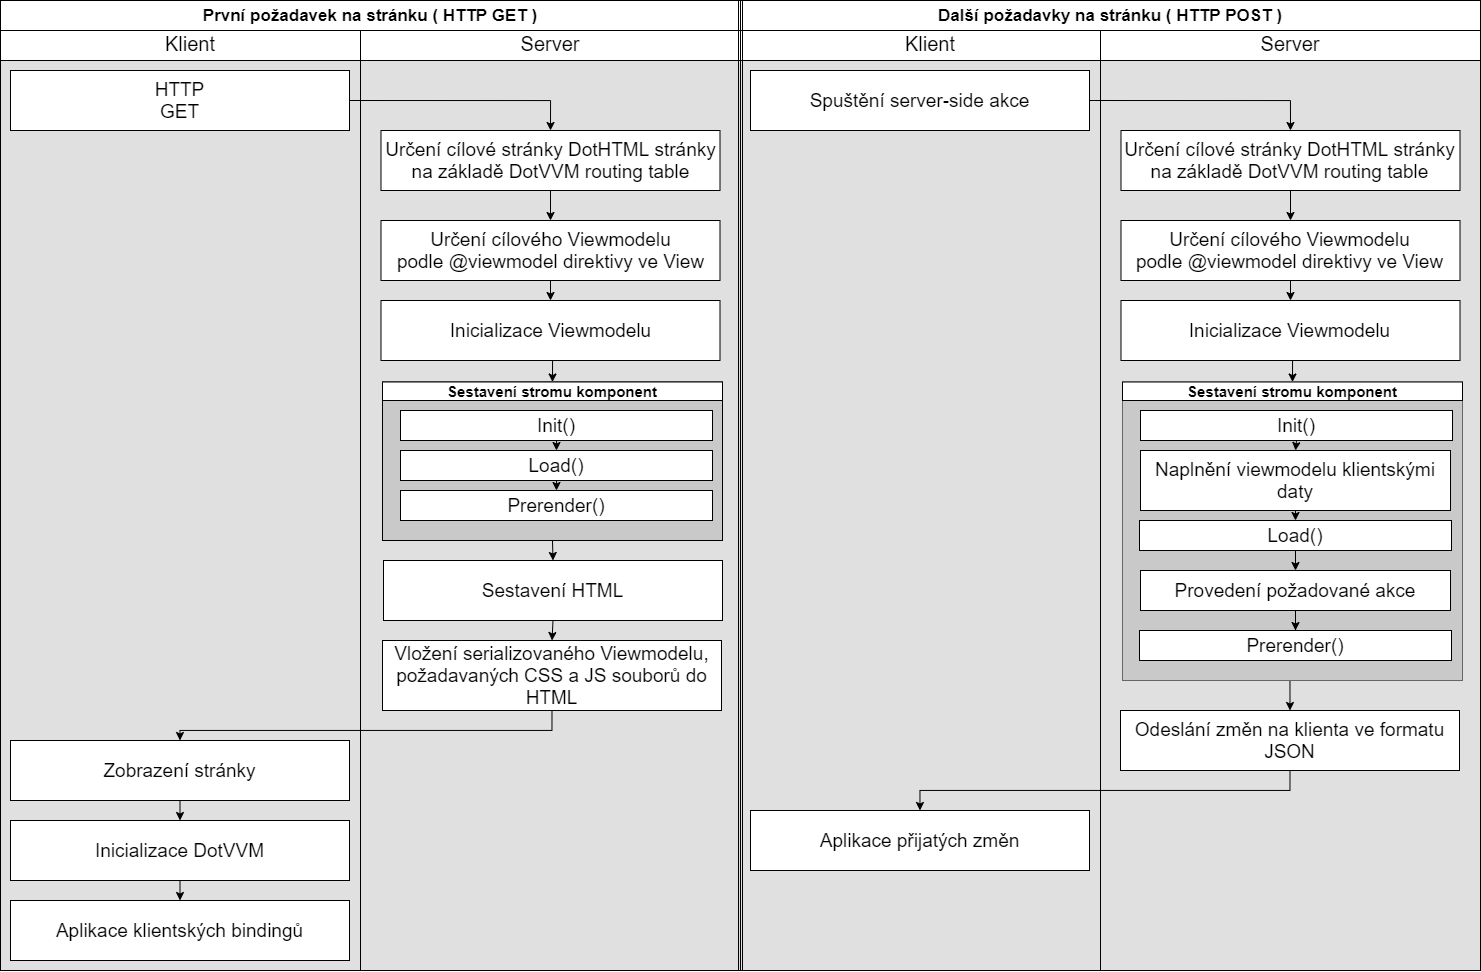
\includegraphics[width=1\textwidth]{obrazky-figures/DotVVM_lifecycle.png}\hfill
	\caption{Popis životního cyklu DotVVM stránek při HTTP GET a POST požadavcích.}
	\label{Get a Post v DotVVM}
\end{figure}

Každé DotHtml je přeloženo do stromové struktury a následně je z tohoto stromu vygenerováno výsledné HTML, které se odešle jako odpověď na klientský dotaz.

\begin{enumerate}
    \item Do příslušného DotVVM presenteru dojde request od klienta. Výběr tohoto presenteru zajišťuje DotVVM routing.
    \item DotvvmViewBuilder sestaví z DotVVM View markapu strom reprezentující dané view. 
    \begin{enumerate}[label*=\arabic*.]
        \item Podle informací obsažených v tomto stromu se do jeho uzlů doplní .net typy, příslušný datakontext a další sémantické informace => vznikne sémantický strom.
        \item Z tohoto sémantického stromu se vytvoří strom komponent. Jednotlivé komponenty jsou reprezentovány jako .net třídy, které popisují, jak pro danou komponentu vytvořit HTML. V tomto stromu jsou reprezentované i normální HTML tagy jako HtmlGenericControl.
    \end{enumerate}
    \item Nastaví se RequestContext\footnote{RequestContext: Objekt obsahující informace o HTTP požadavku.}.
    \item Vytvoření viewmodelu.
    \item Zavolání metody OnPageInitializedAsync na zaregistrovaných filterch typu IViewModelActionFilter\footnote{\label{ActionFilterNote}ActionFilter: Třída implementující rozhraní IActionFilter, která umožnuje provádění dodatečných akcí během kompilace a inicialize DotVVM stránky. }.
    \item Vygenerovanému stromu se nastaví DataContext\footnote{\label{DataContext}DataContext: Reference na objekt ze které se budou brát všechny navázané vlastnosti.}.
    \item Zavolání OnPreInit na jednotlivých komponentách.
    \item Vygenerovanému stromu se nastaví DataContext\footref{DataContext}.
    \item Zavolání Init metody na viewmodelu.
    \item Zavolání OnInit na jednotlivých komponentách.
    \item Zavolání metody OnViewModelCreatedAsync na zaregistrovaných filtrech typu IPageActionFilter\footref{ActionFilterNote}.
    \begin{multicols}{2}
        První request.
        \begin{enumerate}[label*=\arabic*.]
            \item Zavolání Load metody na viewmodelu.
            \item Zavolání OnLoad na jednotlivých komponentách.
        \end{enumerate}
        \begin{description}
        \item 
        \item 
        \item 
        \item 
        \item 
        \item 
        \item 
        \item 
        \item 
        \item 
        \item 
        \item 
        \item 
        \item 
        \end{description}
    \columnbreak
        Postback
        \begin{enumerate}[label*=\arabic*.]
            \item Načtení viewmodelu z příchozího HTTP požadavku.
            \item Zavolání metody OnViewModelDeserializedAsync na zaregistrovaných filterch typu IViewModelActionFilter\footref{ActionFilterNote}.
            \item Validace CSRF Tokenu\footnote{\label{CSRF} CSRF Token slouží k obraně před \textbf{C}ross \textbf{S}ite \textbf{R}equest \textbf{F}orgery útoky.}.
            \item Zavolání Load metody na viewmodelu.
            \item Zavolání OnLoad na jednotlivých komponentách.
            \item Zavolání metody OnCommandExecutingAsync na zaregistrovaných filterch typu ICommandActionFilter\footref{ActionFilterNote}.
            \item Spuštění požadované akce.
            \item Zavolání metody OnCommandExecutedAsync na zaregistrovaných filterch typu ICommandActionFilter\footref{ActionFilterNote}.
        \end{enumerate}
    \end{multicols}
    \item Zavolání PreRender metody na viewmodelu.
    \item Zavolání OnPreRender na jednotlivých komponentách.
    \item Zavolání PreRenderComplete na jednotlivých komponentách.
    \item Vygenerování CSRF tokenu\footref{CSRF}.
    \item Zavolání metody OnViewModelSerializingAsync na zaregistrovaných filterch typu IViewModelActionFilter\footref{ActionFilterNote}.
    
    \item OutputRenderer sestaví výslednou odpověď na klientský požadavek.
    \begin{enumerate}
        \item Nastaví požadované HTTP hlavičky
        \item Zavolá metodu Render na sestaveném view (kořenu stromu), ten pak metodu Render zavolá na svých potomcích.
        \item Zkontroluje se, že došlo k vyrenderování externích prostředků.
        \item Vytvoří nový HtmlWriter, který bude zapisovat do odpovědi.
    \end{enumerate}
    \item Odešle se odpověď na klientský požadavek.
\end{enumerate}

\chapter{Integrace technologie AMP do~DotVVM}
Hlavní myšlenkou vytvoření integrace technologie AMP do již existujících DotVVM stránek bylo,  umožnit napsat celou webovou aplikaci, včetně statických veřejných stránek, v jedné technologii bez toho abychom přišli o rychlost kterou nám čistě statický web nabízí ale kterou při použití webových frameworků částečně ztrácíme.

Aby tato myšlenka v praxi fungovala, je nutné minimalizovat objem změn a konfigurace, kterou musí uživatel udělat, aby jeho stránka využila místo DotVVM technologii AMP. Z tohoto důvodu je použití tohoto rozšíření navrženo tak, aby stránky, které neobsahují žádný technologií AMP zakázaný prvek, fungovaly bez jakýchkoli úprav. V tomto ideálním scénáři by mělo stačit jen označit danou stránku jako stránku s podporou technologie AMP. Po této jednoduché konfiguraci by měla vzniknout verze původní stránky, která nebude na straně klienta používat technologii DotVVM ale technologii AMP.

Aplikace velké části potencionálních uživatelů bohužel nejspíše nebudou splňovat všechny podmínky nutné pro převod do technologie AMP bez jakýchkoliv dodatečných úprav nebo konfigurací. Pro tyto případy je nutné podporovat způsob, jak v rámci View anotovat které části se používají jen v rámci AMP stránky a které jen v rámci DotVVM stránky. Díky možnosti takto specifikovat různé verze pro jednotlivé technologie bude možné se vyhnout nucené úpravě již existující DotVVM stránky jen proto, aby její AMP verze byla validní.

Posledním důležitým aspektem této integrace je umožnit ( ale nevynucovat ) možnost konfigurovat, případně nahradit, jednotlivé komponenty zajišťující převod DotVVM stránky do technologie AMP.

Z těchto poznatků vyplývají základní prvky, které by měl tento projekt splňovat:

\begin{itemize}
\item jednoduché na použití
\item minimalizace potřebného množství zásahů do původních stránek
\item velká míra rozšiřitelnosti
\end{itemize}
\section{Registrace a konfigurace DotVVM.AMP}
Pro správné chování všech prvků DotVVM.AMP je nutné nejdříve zaregistrovat potřebné prostředky do DotVVM a IOC\footnote{IOC: Inversion of Control} kontejneru. API\footnote{Programové rozhraní, které využívají ostatní části aplikace pro kontrolu našeho kódu.} pro registraci DotVVM.AMP je navrženo tak aby se co nejvíce podobalo registračnímu API dalších rozšíření DotVVM\footnote{Nejrozšířenější rozšíření DotVVM jsou balíky komponent DotVVM Bootstrap a DotVVM BusinessPack.}.

\subsection*{Registrace prostředků}
Pro registraci prostředků a komponent, které DotVVM.AMP vyžaduje, se používá zavolání extension metody\footnote{\label{extension}Extension metoda je statická metoda, které je přidána k určitému typo na jiném místě než v rámci jeho definice.} AddDotvvmAmp na typu DotvvmConfiguration. Tuto registraci bych doporučoval provádět v rámci metody Configure v třídě DotvvmStartup.

Tato metoda zaregistruje do DotvvmResourceRepository dva prostředky: AMP CSS boilerplate a AMP JS boilerplate. Tyto prostředky vloží do HTML hlavičky ampem vyžadovaný Css a Js kód.

\subsection*{Registrace AMP komponent}
V rámci volání extension metody\footref{extension} AddDotvvmAmp se také zaregistrují všechny AMP komponenty, které jsou v namespace DotVVM.AMP.AmpControls jako DotVVM komponenty s prefixem amp\footnote{Jejich použití bude tedy <amp:\textit{JMÉNO} \ldots /> . }.

\subsection*{Registrace používaných tříd do IOC kontejneru}

Kvůli požadavku na snadnou modifikaci defaultního chování jednotlivých částí DotVVM.AMP bylo zapotřebí co nejvíce omezit vznik pevných závislostí mezi jednotlivými částmi knihovny. Tento problém jsem se rozhodl vyřešit pomocí DI\footnote{\label{DI}DI: Dependency Injection}.

Všechny závislosti jednotlivých komponent jsou definovány ne konkrétní implementací ale pouze pomocí rozhraní. IOC kontejner poté při vytváření instance doplní ke každému požadovanému rozhraní příslušnou implementaci. To jakou implementaci (a to jestli má vytvářet nebo znovu používat dané instance) je definováno v rámci registrací komponent do IOC kontejneru.

Tato registrace se provádí v rámci volání extension metody\footref{extension} AddDotvvmAmpSupport na typu IDotvvmServiceCollection.

\subsection*{Konfigurace DotVVM.AMP}
Veškerá konfigurace DotVVM.AMP se uchovává v rámci třídy DotvvmAmpConfiguration. V rámci celé webové aplikace by vždy měla existovat jen jedna instance této třídy. Tímto způsobem je zjištěno, že všechny stránky se chovají stejně. Konfigurace se dá pomyslně rozdělit na tři části: instance sdílených vlastností, globální nastavení a nastavení chování jednotlivých typů validací.

\subsubsection{Sdílené instance}
\begin{itemize}
    \item \textit{ControlTransforms} \newline
Registr obsahující registrace jednotlivých transformací DotVVM komponenty na AMP komponentu.
    \item \textit{RouteManager}\newline
Třída obsahující logiku pro pojmenovávání a správu cest na jednotlivá AMP stránky.
    \item \textit{ExternalResourceMetadataCache}\newline
Cache obsahující metadata (například rozměry) o externích zdrojích (primárně obrázcích).
\end{itemize}

\subsubsection{Globální nastavení}
\begin{itemize}
    \item \textit{TryToDetermineExternalResourceDimensions} \newline
    Určuje zda v případě nalezení obrázku, u kterého neznáme jeho velikost, dojde k pokusu zjistit jeho rozměry.
    \item \textit{StyleRemoveForbiddenImportant}\newline
    Určuje zda se mají být z CSS kódu odstraněny AMPem zakázané modifikátory !important.
    \item \textit{AmpJsUrl}\newline
    Určuje jaká zdroj poviného AMP Js. Změnou tohoto parametru můžeme změnit používanou verzi technologie AMP.
    \item \textit{MaximumAmpCustomStylesheetSize}\newline
    Určuje jaká velikost v bytech vlastního CSS bude ještě akceptována.
\end{itemize}


\subsubsection{Nastavení validací} \label{validationModes}
Všechny validace podporují dva režimy:
\begin{itemize}
    \item Throw \newline
    Při první chybě překlad ukončem a dojde ke vzniku záznamu v logu a vyjímky, která danou chybu popisuje.
    \item LogAndIgnore \newline
    Při chybě bude daná chyba zaznamenána, ale kompilace bude pokračovat dále. Element (nebo jeho část) obsahující chybu bude ve většině případů vynechán.
\end{itemize}
Kvůli zajištění větší granulity jsou validace v různých kontextech nastavovány samostatně pomocí těchto vlastností v rámci DotvvmAmpConfiguration: 
\begin{itemize}
    \item \textit{AttributeHandlingMode} \newline
    Nastavení chování při nalezení nevalidního HTML atributu.
    \item \textit{KnockoutHandlingMode}\newline
    Nastavení chování při nalezení knockout bind atributu (xml:\textit{*}).
    \item \textit{HtmlTagHandlingMode}\newline
    Nastavení chování při nalezení nevalidního HTML tagu.
    \item \textit{StylesHandlingMode}\newline
    Nastavení chování při nalezení nevalidního CSS.
    \item \textit{UnsupportedControlPropertiesHandlingMode}\newline
    Nastavení chování při nalezení nevalidně nastavené DotVVM komponenty.
\end{itemize}

Veškerá nastavení by měla probíhat výlučně v rámci volání metody AddDotvvmAmpSupport. Této metodě je možné jako parametr předat Action<DotvvmAmpConfiguration>\footnote{Action<DotvvmAmpConfiguration> : Anonymní metoda s návratovým typem void, která jako jediný parametr dostane instanci DotvvmAmpConfiguration}. Tato Action by měla sloužit jako jediné místo, kde bude zasahováno do DotvvmAmpConfiguration. Takto provedené úpravy konfigurace budou aplikovány hned jakmile si nějaká část DotVVM.AMP poprvé vyžádá přístup ke konfiguraci.

\begin{lstlisting}[language=c#, caption=Registrace DotvvmAmpConfiguration,label=RegAmpConfig,captionpos=t]
serviceCollection.Services.AddSingleton<DotvvmAmpConfiguration>(provider =>
{
    var registry = provider.GetService<IAmpControlTransformsRegistry>();
    var routeManager = provider.GetService<IAmpRouteManager>();
    var logger = provider.GetService<ILogger>();
    var resourceMetadataCache =
        provider.GetService<IAmpExternalResourceMetadataCache>();
    var config =
        new DotvvmAmpConfiguration(registry, routeManager,resourceMetadataCache);
        
    RegisterTransforms(config, logger);
    modifyConfiguration?.Invoke(config);
    return config;
});
\end{lstlisting}
\section{Rozšíření DotVVM routing table}
Jelikož DotVVM.AMP nenahrazuje již vytvořené DotVVM stránky, ale jen k ni vytváří jejich AMP verzi, tak se jako nejlepší místo pro definici, které stránky budou přeloženy do technologie AMP, jeví kód provádějící registrace DotVVM stránek do DotVVMRouteTable (příklad registrace DotVVM stránky je uveden v ukázce \ref{RegDotVVMPage}).

\begin{lstlisting}[language=c#, caption=Registrace DotVVM stránky do DotvvmRouteTable,label=RegDotVVMPage,captionpos=t]
config.RouteTable.Add("Default", "index", "Views/Default.DotHtml");
\end{lstlisting}

Pro jednoduché stránky nepotřebuji od uživatele jiné informace, které jsou povinné v rámci registrace klasické cesty.
Tudíž se jako ideální řešení způsobu registrace jeví přidání DotVVM.AMP pomocí nahrazení volání metody Add nad DotvvmRouteTable extension metodou AddWithAmp, která se volá nad stejným typem a má skoro stejné vyžadované parametry. Takto upravená registrace do DotVVM route table je uvedena v ukázce \ref{RegAmpRoute}.

\begin{lstlisting}[language=c#, caption=Registrace AMP stránky do DotvvmRouteTable,,label=RegAmpRoute, captionpos=t]
config.RouteTable.AddWithAmp("Default", "index", "Views/Default.DotHtml",config);
\end{lstlisting}

Jediné co se na signatuře metody změnilo (kromě jejího názvu) je nový parametr vyžadující instanci DotVVMConfiguration.

Pro náročnější scénáře je možné jako parametry předat defaultní hodnoty url parametrů jak DotVVM stránky tak její AMP verze. Také je možné specifikovat, který DotVVM presenter bude použit pro DotVVM stránku a který pro její AMP verzi. Specifikace presenteru umožňuje například podporu lokalizací pomocí LocalizablePresenter (resp DotvvmAmpLocalizablePresenter pro AMP variantu).

Zavolání metody AddWithAmp vygeneruje dvě odlišné DotVVM cesty, jednu pro původní DotVVM stránku a druhou pro její AMP verzi.\newline
Generování těchto cest probíhá následovně:
\begin{itemize}
    \item Získání AMP konfigurace z IOC kontejneru.
    \item Vygenerování názvu  DotvvmRoute pro AMP verzi pomocí AmpRouteManageru.\newline
    V základu mají cesty tento formát: \textit{PŮVODNÍ-NÁZEV}-amp .
    \item Vygenerování URL  pro AMP verzi pomocí AmpRouteManageru.\newline
    V základu má tento formát: \textit{amp/PŮVODNÍ-URL} .
    \item Pokud nejsou nastaveny separátní defaultní hodnoty pro AMP verzi, tak se použijí defaultní hodnoty pro původní verzi.
    \item Přidání cesty pro DotVVM stránku.
    \item Přidání cesty pro AMP stránku.
    \item Registrace překladu do AmpRouteManageru.\newline
    Tato informace se používá pro nalezení DotVVM varianty AMP stránky a naopak.
\end{itemize}

\section{AmpPresenter}
DotvvmPresenter funguje jako centrální bod, který kontroluje průběh zpracování requestu na DotVVM stránku. Tato třída má jako závislosti (které jsou inicializovány pomocí DI\footref{DI}) všechny části DotVVM infrastruktury. Z tohoto důvodu je vlastní DotvvmPresenter ideální místo pro nahrazení DotVVM závislostí jejich DotVVM.AMP verzemi.

AmpPresenter funguje jako dekorátor defaultního DotvvmPresenteru. Tento dekorátor modifikuje dvě části původního chování.

\subsection*{Nahrazení původních závislosti}
Závislosti na defaultní DotVVM třídy jsou nahrazeny jejich AMP variantami v rámci konstruktoru\footnote{Constructor Injection: Závislosti vyžadované v rámci konstruktoru jsou doplněny patřičnými instancemi dle pravidel DI kontejneru.}.

\begin{itemize}
    \item IDotvvmViewModelBuilder => IAmpDotvvmViewBuilder \newline
    AmpViewBuilder rozšiřuje DefaultDotvvmViewBuilder o podporu transformací během sestavování výsledného stromu komponent.
    \item IOutputRenderer => IAmpOutputRenderer \newline
    AmpOutputRenderer nahrazuje HtmlWriter za AmpHtmlWriter. AmpHtmlWriter umožňuje provádět poslední validace před vygenerováním HTML.
\end{itemize}

\subsection*{Registrace resource preprocesorů}
Kvůli nutnosti upravovat externí prostředky (hlavně CSS) je nutné pro každý request zaregistrovat dvě třídy typu IResourceProcessor do ResourceManageru.
\begin{itemize}
    \item AmpCustomCssResourceProcessor \newline
    AmpCustomCssResourceProcessor zajišťuje spojení všech CSS do jednoho\footnote{V některých případech je možné, že vzniknou dva inline styly.} inline stylu.
    \item AmpResourcesProcessor \newline
    AmpResourcesProcessor vyfiltruje všechny nepovolené prostředky.
\end{itemize}

\subsection*{DotvvmAmpLocalizablePresenter}
Druhým presenterem, který je v rámci DotVVM.AMP implementován, je DotvvmAmpLocalizablePresenter. Tento presenter je AMP variantou na DotVVM LocalizablePresenter.
Účel localizable presenteru je nastavit do  CultureInfo.CurrentCulture a CultureInfo.CurrentUICulture uživatelem vyžádaný jazyk\footnote{Vyžadovaný jazyk je nejčastěji zadán v rámci nepovinného URL parametru.}. Po nastavení jazyka je další zpracování požadavku delegováno na defaultní DotvvmPresenter.

Jediný rozdíl v DotvvmAmpLocalizablePresenteru oproti LocalizablePresenteru je že namísto toho, aby se delegovalo zpracování další requestu na DotvvmPresenter, tak se zpracování deleguje na AmpPresenter.

\section{Rozšíření DotHtml}

Některé technologií AMP vyžadováné prvky jsou v rámci DotVVM.AMP řešené náhradou stávájící komponenty (HTML elemetntu,...) za separátní komponentu.  Mimo interní komponenty existují také komponenty, které lze použít v rámci DotHtml. Pomocí těchto komponent lze například přidat do již existujícího HTML prvky, 
 které budou obsažené jen v AMP verzi (nebo jen v DotVVM verzi).
 
\subsection*{Interní komponenty}
Většina komponent v DotVVM.AMP jsou interní komponenty použité jen pro účely transformací. Interní komponenty nelze používat v rámci DotHtml.

\subsubsection*{AmpBody}
DotVVM se v rámci renderování HtmlGenericControl\footnote{Každý HTML tag (ne DotVVM komponenty) je v rámci stromu komponent reprezentován jako HtmlGenericControl.}, která má nastaven svůj HTML tag na body, pokusí vyrenderovat všechny externí prostředky. Tomuto chování ale musíme v rámci DotVVM amp zabránit, protože tyto prostředky defaultně obsahují javascriptové soubory nutné pro běh DotVVM.

Tento mechanismus bohužel není navržen tak, aby bylo možné tomuto chování jednoduše zabránit. Z tohoto důvodu jsem se na tomto místě musel uchýlit k využití reflection\footnote{Reflection například umožňuje dynamicky za běhu měnit hodnoty jinak nedostupných vlastností (například privátní vlastnosti).}. Při překladu první stránky se získá informace o vlastnosti\footnote{ProperetyInfo: Informace o vlastnosti sloužící pro nastavení nebo získání hodnoty pomocí reflection.} BodyRendered na typu ResourceManager. Tato informace o vlastnosti se následně využije pro nastavení této vlastnosti na hodnotu true, což zabrání renderování nechtěných prostředků.

\subsubsection*{RouteLink}
Komponenta RouteLink rozšiřuje chování defaultního RouteLinku logiku, která zajišťuje použití Amp varianty odkazované stránky namísto původní DotVVM stránky. Pokud AMP varianta této stránky neexistuje, tak je použita původní stránka.

Pro vyhledání AMP varianty se používá AmpRouteManager. AmpRouteManager obsahuje tabulku. která eviduje, jaké DotVVM stránky mají AMP verzi. Registrace do této tabulky vznikají při registraci cest do DotVVM route table.

\subsubsection*{AmpLinkToAnotherVersion}
AmpLinkToAnotherVersion je varianta na AMP RouteLink. Tato komponenta přidává odkaz na~původní DotVVM stránku (nebo naopak z DotVVM stránky na její AMP verzi). Tato komponenta se používá místo komponenty AMP RouteLink z důvodu nutnosti správně určit URL parametry pro původní stránku.

Pokud původní DotVVM stránka má defaultní parametry a pro přístup na aktuální stránku byly použity defaultní parametry pro AMP verzi, tak vygenerovaný odkaz vede na URL používající defaultní parametry DotVVM stránky. To znamená, pokud byly parametry defaultní tak defaultní zůstanou, jen se použijí defaultní parametry pro správnou verzi dané stránky.

Pokud výše uvedené pravidlo splněno není, tak se použijí aktuální parametry.

\subsubsection*{AmpRepeater a AmpGridView}
AmpRepeater a AmpGridView v DotVVM verzi používají vnitřní šablony.

\begin{itemize}
    \item Komponenta Repeater zduplikuje tuto šablonu pro všechny prvky v jejím zdroji dat\footnote{DataSource: zdroj dat pro danou komponentu}.Každý takto zduplikovaný prvek obsahuje data která jsou získána z daného prvku.
    \item Komponenta GridView obsahuje v šabloně definice (šablony) jednotlivých sloupců tabulky, které jsou pak použity pro vykreslení jednotlivých řádků.
\end{itemize}

Obsah těchto šablon není ve stromu komponent během transformací, a proto se na něj transformace neaplikují. Z tohoto důvodu je nutné všechny transformace aplikovat dodatečně a tudíž jsou defaultní komponenty Repeater a Gridview nahrazeny jejich AMP variantami.

\subsection*{Amp komponenty}
 Některé komponenty v DotVVM.AMP jsou určené i k použití v rámci DotHtml.
 \subsubsection{Image}
 Tato komponenta reprezentuje náhradu za HTML img tag. Této komponentě můžeme nastavit běžné vlastnosti obrázku jako například velikost a zdroj, ale také i vlastnosti specifické pro amp-img. Hlavní z těchto nových vlastností je atribut Layout. Tento atribut určuje, jak bude výsledný obrázek napozicován v rámci AMP stránky.
 
 Z důvodu modifikaci URL oproti původní stránce je v rámci generování HTML pro obrázek nutné zajistit, aby zdroj obrázku obsahoval absolutní cestu. Pokud je detekována relativní cesta, dojde k její transformaci na cestu absolutní pomocí doplnění kořenové cesty, které se získá z příchozího požadavku.
 
 Hodnota tohoto atributu Layout také ovlivňuje, zda je nutné, aby obrázek měl zadanou výšku anebo šířku. Pokud není Layout nastaven tak je nutné, aby obrázek měl výšku i šířku. V případě že velikost obrázku nastavená není, a v rámci DotvvmAmpConfiguration je nastavena vlastnost TryToDetermineExternalResourceDimensions na hodnotu true, tak se pokusím velikost obrázku zjistit.
 
 Detekce velikosti obrázku se provádí v rámci třídy AmpExternalResourceMetadataCache. Obrázek se nejprve stáhne a pak se pokusím vyčíst jeho velikost. Tento mechanismus bohužel selže pro vektorové obrázky\footnote{Vektorové obrázky nemají specifikovanou velikost.}. Pro každý obrázek (pro každou URL) je detekce velikosti provedena pouze jednou. Pro každý další dotaz se použije dříve získaná hodnota.
 
 \subsubsection{Exlude a Include}
 Pro kontrolu, zda se nějaká stránka má vyrenderovat jen v rámci AMP verze nebo jen v rámci původní Dotvvm stránky, lze použít komponenty Exlude a Include.
 
 Obsah Exclude komponenty se vyrenderuje jen v původní stránce a obsah Include komponenty jen v AMP verzi. Pro tento účel lze také použít attached propertu\footnote{Attached properties: Vlastnosti které lze použít v rámci jakékoliv komponenty.} AMP.Exclude.
 
 Detekce, toho zda se komponenta nachází v AMP nebo původní verzi stránky, je založena na tom, že pouze v AMP verzi probíhají transformace. Na detekci, zda proběhly transformace, se používá transformace, která doplňuje instanci DotvvmAmpConfiguration do vlastnosti Configuration v rámci dekorátorů. Pokud je vlastnost Configuration prázdná (hodnota je null), tak to znamená že se nenacházíme na AMP verzi stránky.
 
 To jestli dojde nebo nedojde k vygenerování obsahu těchto stránek se provádí pomocí podmíněného přeskočení fáze RenderContents dané komponenty.
 
\section{Sestavení Dotvvm View}
O sestavení Dotvvm View se v klasických DotVVM stránkách stará DefaultDotvvmViewBuilder. Tato třída nejprve načte příslušné DotHTML a z něj pak sestaví strom komponent. V případě, že stránka používá šablony, tak se v rámci sestavení stromu komponent načte a zpracuje DotHTML i těchto stránek. Na konci tohoto procesu vznikně DotVVM komponenta  DotvvmView, která reprezentuje strom komponent.

V rámci DotVVM.AMP se pro sestavení view používá AmpViewBuilder. Tato třída dekoruje IDotvvmViewBuilder. AmpViewBuilder nejprve nechá původní implementaci IDotvvmViewBuilder sestavit strom komponent pro původní DotVVM stránku a následně na takto sestavený strom začne aplikovat transformace. Proces výběru a aplikace transformací je znázorněn v ukázce \ref{ApplyTransforms}. 
\begin{lstlisting}[language=c#, caption= Ukázka aplikace transformací ,label=ApplyTransforms,captionpos=t]
public void ApplyTransforms(DotvvmControl root,IDotvvmRequestContext context)
{
    ApplyTransforms(root.GetAllDescendants().ToList(), context);
}

public void ApplyTransforms(List<DotvvmControl> allControls, IDotvvmRequestContext context)
{
    foreach (var control in allControls)
    {
        GetTransform(control)?.Transform(control, context);
    }
}
\end{lstlisting}
\subsection*{Transformace}
Transformace jsou třídy implementující IControlTransform. Tyto třídy mají za úkol transformovat strom komponent reprezentující DotVVM stránku, na strom komponent reprezentující AMP stránku. Transformace dělíme do několika kategorií: klasické, validační a nahrazující. To jestli je možné danou transformaci použít, zjistíme pomocí metody CanTransform, kterou musí každá transformace implementovat.
\subsubsection{Klasické transformace}
    Klasické transformace dědí z ControlTransformBasem. Jsou to transformace, které mohou pouze měnit nastavení dané komponenty. Samotná transformace probíhá v několika krocích:
    \begin{enumerate}
        \item Rozhodnutí, zda by tato komponenta měla být zahrnuta ve výsledném stromu komponent.\newline
        V případě, že je na komponentě nastaveno například Amp.Exclude na hodnotu true, dojde k jejímu vyřazení ze stromu komponent a dále se již v transformaci nepokračuje.
        \item Provedení BeforeTransform metody.\newline
        Tuto metody aktálně žádná z transformací neimplementuje. Metoda existuje z důvodu pozdější rozšiřitelnosti.
        \item Provedení TransformCore metody.\newline
        Každá transformace tuto metodu musí implementovat. V této transformaci by měly proběhnout všechny úpravy. 
        \item Nastavení vyžadovaných vlastností.\newline
        Všechny AMP komponenty musí být vyrenderovány již na serveru. Tato metoda nastavení RenderSettings.ModeProperty na hodnotu RenderMode.Server.
        \item Aplikace attached properties.\newline
        V tomto kroku dojde k přidání AMP atributů fallback nebo placeholder, pokud je komponenta vyžaduje.
        \item Provedení AfterTransform metody.\newline
        Metoda existuje z důvodu pozdější rozšiřitelnosti. Některé transformace v rámci této metody provádějí finální úpravy komponenty.
    \end{enumerate}
\subsubsection{Validační transformace}
    Validační transformace jsou rozšířením klasických transformací. Jsou to transformace, které dědí z ControlValidatorTransformBase. Validační transformace provádí ověření, zda je danou komponentu v jejím aktuálním nastavení možné použít v rámci AMP stránky. Tyto transformace v rámci metody TransformCore provedou validaci požadovaných vlastností. Pokud daná vlastnost není validní, tak dojde k výjimce nebo k vynechání dané komponenty a zalogování chyby (záleží na nastavení UnsupportedControlPropertiesHandlingMode).
\subsubsection{Nahrazující transformace}
    Nahrazující transformace jsou rozšířením validačních transformací. Jsou to transformace, které dědí z ControlReplacementTransformBase. Nahrazující transformace nahradí jednu komponentu za jinou v rámci TransformCore metody. V rámci nahrazení dojde ke zkopírování všech atributů a vlastností. Při nahrazení komponenty je nutné přenést všechny potomky dané komponenty a také je důležité správně nastavit odkaz na rodičovskou komponentu a původní komponentu ze stromu odebrat. Kód zajištující nahrazení komponenty je uveden v ukázce \ref{ControlReplace}.
    
    \begin{lstlisting}[language=c#, caption= Nahrazení jedné DotVVM komponenty za jinou. ,label=ControlReplace,captionpos=t]
public void ReplaceControl(DotvvmControl currentControl, DotvvmControl newControl)
{
    var parent = currentControl.Parent as DotvvmControl;
    DotvvmControl[] children = new DotvvmControl[currentControl.Children.Count];
    currentControl.Children.CopyTo(children, 0);

    if (parent != null)
    {
        var childIndex = parent.Children.IndexOf(currentControl);

        parent.Children.Remove(currentControl);
        parent.Children.Insert(childIndex, newControl);
    }
    currentControl.Children.Clear();
    currentControl.Parent = newControl.Parent;
    newControl.Children.Add(children);
}

\end{lstlisting}

\section{Css infrastruktura}
AMP zakazuje externích CSS styly a omezuje styly vložené do stránky na max 75kB vlastního CSS v jediném HTML style tagu. Jedinou výjimkou pro toto pravidlo je maximálně 500kb CSS keyframes, které můžou být obsaženy v samostatném style elementu.

Díky těmto pravidlům je nutné nejprve všechny externí a embedované\footnote{embedované: Vložené přímo na stránku.} styly spojit do jediného CSS kódu a ten následně rozdělit na CSS keyframes a zbytek. Spojení probíhá v několika fázích.
\subsection*{Modifikace stromu komponent}
V rámci aplikace transformací dochází odebrání všech embedovaných stylů a odkazů na externí styly. Tyto styly jsou odebrány ze stromu komponent a přidány do vyžadovaných prostředků.

\subsection*{Sjednocení CSS v rámci externích prostředků}
V průběhu vyhodnocování externích prostředků dochází k aplikaci ResourceProcessorů\footnote{ResourceProcessor: Třída implementující IResourceProcessor. Tato třída v rámci metody Process bere jako parametr množinu externích prostředků a vrací množinu externích prostředků. Tuto třídu lze tedy použít pro modifikaci (například přidání nebo odebrání) externích prostředků. ResourceProcessory jsou při aplikaci volány postupně => Výsledky jednoho dostane na vstupu následující ResourceProcessor.}. Pro sjednocení CSS se používá AmpCustomCssResourceProcessor, který je registrován v~rámci DotvvmAmpPresenteru. Tento processor vždy když nalezne CSS prostředek, tak jej uloží do AmpStylesheetResourceCollection. Když projde všechny vyžadované prostředky, tak vrátí ještě dva další prostředky: AmpCustomStylesheetResource a AmpCustomStylesheetResource.

\subsection*{Vygenerování amp-custom a amp-keyframes elementů}
Během vykreslení prostředku AmpCustomStylesheetResource nebo AmpCustomStylesheetResource dojde k vygenerování výsledného CSS. O generování CSS se stará AmpStylesheetResourceCollection. Pokud AmpStylesheetResourceCollection již někdy generovalo daný CSS kód, tak vrátí původní verzi, jinak dojde k vygenerování CSS pro amp-custom a CSS  pro amp-keyframes

\subsubsection*{Generování CSS}
\begin{enumerate}
    \item Asynchronně se stáhnout všechny požadované CSS.
    \item Všechny CSS kódy se spojí do jediného CSS.
    \item Dojde k ověření na předčastné ukončení.
    \item CSS se naparsuje.\footnote{Parsování CSS se provádí pomocí knihovny ExCSS-Core. \newline https://github.com/HockeyJustin/ExCSS_Core.}
    \item Pokud je v rámci DotvvmAmpConfiguration nastavena vlastnost StyleRemoveForbiddenImportant na true, tak dojde k odstranění všech CSS !important anotací. 
    \item Naparsovaný CSS dokument se rozdělí na CSS Keyframes a ostatní.
    \item Obě výsledné CSS projdou minifikací.\footnote{Minifikace: odstranění všech přebytečných znaků pro účel snížení velikosti. \newline Pro minifikaci CSS se používá kód publikovaný Madsem Kristensenem na jeho blogu.\newline https://madskristensen.net/blog/efficient-stylesheet-minification-in-c}
\end{enumerate}

\section{Sestavení finální stránky}
Když proběhnou veškeré transformace na stromu komponent a jsou připraveny sjednocené CSS prostředky, dochází k vygenerování finálního HTML. Za tento úkon je v rámci klasické DotVVM stránky zodpovědný HtmlWriter. HtmlWriter obsahuje mimo jiné metody pro přidávání různých html atributů, vygenerování počátečního a koncového html tagu a generování čistého textu nebo html kódu. Každá komponenta dostane instanci IHtmlWriter v rámci své Render fáze a využívá tuto třídu pro sestavení výsledného HTML.

V rámci DotVVM amp jsem HtmlWriter využil jako místo ze kterého se provádí finální validace. AmpHtmlWriter dekoruje HtmlWriter a každé z jeho volání obaluje kontrolou na validnost požadovaného konstruktu. Pokud validace tedy selže, tak se daný konstrukt nevygeneruje. Pokud takto dojde k přeskočení počátečního tagu, tak je následně nutné ignorovat vše až do příslušného ukončovacího tagu. Kód zajištující toto chování je uveden v ukázce \ref{AmpHtmlWriter}.


\begin{lstlisting}[language=c#, caption=Metoda RenderBeginTag na třídě AmpHtmlWriter ,label=AmpHtmlWriter,captionpos=t]
public virtual void RenderBeginTag(string name)
{
    if (validator.CheckHtmlTag(name,Attributes))
    {
        Attributes.Clear();
        writer.RenderBeginTag(name);
    }
    else
    {
        StartTagSkipped = true;
    }
}
\end{lstlisting}

\section{Validace}
Mnoho DotVVM aplikací používá i v rámci svých úvodních (a jiných jednoduchých) stránek některou z forem obsahu, které nejsou technologií AMP podporované. Nejčastější takové prvky jsou kontaktní formuláře, webové galerie vyžadující javascript nebo jiné prvky, které bohužel nelze jednoduše převést do technologie AMP.
Pro tyto případy je nutné dát uživatelům vědět, jaké části jejich webových stránek nemohou být převedeny do technologie AMP a z jakého důvodu. Z diskuze s lidmi, co vyvíjí v technologii DotVVM, vyplynulo, že část chce jen vědět, že se na stránce vyskytují nevalidní prvky (spolu s informací o místě a typu problému), ale i přesto chtějí, aby stránka byla do technologie AMP převedena. A to i v případě že by nevalidní elementy nebo jejich části byly v průběhu překladu vynechány. Druhá skupina uživatelů preferuje čistě opačný přístup. Tato skupina chce, aby ve chvíli, kdy je nalezen nevalidní element, došlo k výjimce a nedocházelo tak k tomu, že z výsledné stránky budou vynechány některé elementy.

Z tohoto důvodu si uživatel pro každou skupinu validačních pravidel může nastavit, jak se má validace chovat v případě nalezení nevalidního prvku. Pro každou skupinu existují dva módy: Throw a Log and Ignore. Bližší popis jednotlivých módů lze nalezt v rámci popisu nastavení validací v této kapitole.

V rámci generování HTML pro některé komponenty se stává, že komponenta i zkusí přidat klientský DataBind atribut. V rámci AMP stránek bohužel tyto atributy nemohou fungovat, protože javascript, který tyto atributy zpracovává, na není možné do stránky vložit. Některé tyto dataBind výrazy nám ale v rámci AMP stránek nevadí, protože zajišťují aktualizaci hodnot při postbacku. Namísto toho. aby v těchto případech nastala výjimka (v případě že je pro danou validační skupinu její chování nastaveno na Throw), tak jen zalogujeme upozornění, že byl tento atribut vynechán.

\section{Rozšiřitelnost}
Technologie AMP v základu obsahuje jen tři vestavěné komponenty: amp-layout, amp-image a amp-pixel \cite[Ch.\ 3, p.\ 160]{VzhuruDoAMP}. Tyto tři komponenty by měly pokrýt potřeby pro vytvoření úplně základní stránky. Pokud ale chceme pokročilé komponenty, na které jsme zvyklí ze světa plnohodnotných webových stránek, jako například fotogalerii nebo youtube video, tak musí sáhnout po někté z rozšiřujících komponent.

Aktuálně je v rámci technologie AMP dokumentace k 240 komponentám. V rámci DotVVM.AMP jsou ale podporovány jen výše zmíněné tři komponenty. Pro přidání podpory pro další komponenty je možné pomocí vytvoření vlastní transformace a případně i vlastní komponenty.

Pokud bychom chtěli přidat podporu pro komponentu amp-iframe\footnote{amp-iframe: https://amp.dev/documentation/components/amp-iframe/?format=websites}, tak musíme nejdříve vytvořit DotVVM komponentu \footnote{Tutoriál na tvorbu komponent lze nalézt v rámci DotVVM dokumentace v sekci Control Development.\newline https://www.dotvvm.com/docs/tutorials/control-development-code-only-controls/2.0}, kterou nahradíme všechny iframe na stránce. Tato komponenta bude obsahovat všechny vlastnosti, které budeme chtít podporovat. V případě amp-iframe to jsou:
\begin{itemize}
    \item src\newline
    Odkaz na cílovou stránku.
    \item sandbox\newline
    Nastavení izolace a bezpečnostních pravidel pro daný iframe.
    \item Standardní atributy AMP elementů.\newline
    Tyto atributy obsahuje bázová třída AmpControl, takže stačí, když ji podědíme.
    \item Další atributy standardního HTML iframe.
\end{itemize}

Dále budeme do stránky potřebovat vložit odkaz na požadovaný javascript. Toto uděláme stejně jako kdybychom potřebovali přiložit jakýkoliv jiný prostředek k DotVVM komponentě. Zaregistrujeme prostředek, který vyrenderuje potřebný script HTML tag do DotVVMResourceManageru a ten v rámci OnInit metody přidáme jako required resource.

Jako poslední krok musíme vytvořit transformaci, která všechny HtmlGenericControl s tagem iframe na stránce nahradí za náš iframe a zkopíruje jeho atributy do vlastností, které máme v rámci naší DotVVM komponenty. Pokud bychom nechtěli kopírovat atributy, ale přesto využívat výhody Dotvvm properties, tak můžeme upravit getter příslušných vlastností podobně jako v ukázce \ref{GetPropertyValueOrAttribute}.  Tato transformace by měla dědit z ControlReplacementTransformBase. Bázová třída za nás vyřeší nahrazení nové komponenty ve stromu komponent a nakopíruje všechny DotVVM properties a atributy na novou komponentu. Výsledná transformace by mohla vypadat podobně jako ukázka kódu  \ref{AmpIframe}. Poslední zbývající krok je zaregistrovat naši transformaci do AmpControlTransformRegistry. Tuto registraci můžeme udělat v rámci volání extension metody AddDotvvmAmpSupport nad typem IDotvvmServiceCollection. Příklad této registrace je uveden v ukázce kódu \ref{TransformRegistration}.
\begin{lstlisting}[language=c#, caption=Ukázka možné implementace tranformace pro iframe,label=AmpIframe,captionpos=t]
public class IframeTransform : ControlReplacementTransformBase
{
 public IframeTransform(
                         DotvvmAmpConfiguration ampConfiguration,
                         ILogger logger = null
                       ) : base(ampConfiguration, logger)
 {
 }

  public override bool CanTransform(DotvvmControl control)
  {
     return control is HtmlGenericControl generic &&
            generic.TagName == "iframe";
  }

  protected override DotvvmControl CreateReplacementControl(DotvvmControl control)
  {
      return new AmpIframe();
  }
}
\end{lstlisting}

\begin{lstlisting}[language=c#, caption=Možný způsob jak se vyhnout kopírování HTML atributů do DotVVM property.r ,label=GetPropertyValueOrAttribute,captionpos=t]
public virtual void RenderBeginTag(string name)
{
        public string Src
        {
            get { return GetPropertyValueOrAttribute(SrcProperty, "src"); }
            set { SetValue(SrcProperty, value); Attributes.Remove("src"); }
        }
}
\end{lstlisting}

    \begin{lstlisting}[language=c#, caption=Ukazka možné implementace tranformace pro iframe,label=TransformRegistration,captionpos=t]
public class IframeTransform : ControlReplacementTransformBase
{
    options.AddDotvvmAmpSupport((configuration, logger) =>
    {
        configuration.ControlTransforms.Register(
                new IframeTransform(configuration,logger));
    });
}
\end{lstlisting}

\chapter{Postup integrace překladu stávajících DotVVM stránek do technologie AMP}
V této kapitole popíši postup, jak DotVVM.AMP použít pro přidání AMP verze k již existující DotVVM stránce v rámci reálné webové aplikace. V rámci této ukázky použiji DotVVM.AMP ve verzi 0.1.0.7\footnote{\label{nuget}Knihovna DotVVM.AMP ve verzi 0.1.0.7 je veřejně dostupná na nuget.org.\newline
https://www.nuget.org/packages/DotVVM.AMP/0.1.0.7}. Jako aplikaci, na které budu převod do AMP prezentovat, jsem zvolil webovou aplikaci, která slouží pro prezentaci portfolia. Konkrétně jsem zvolil stránku, která obsahuje detail projektu. Tuto aplikaci (a konkrétní stránky v rámci aplikace) jsem zvolil z toho důvodu, že je dynamicky generovaná\footnote{View je napsáno obecně pro jakýkoliv projekt a specifické informace o dané referenci jsou doplněné v rámci modelu. }, ale přesto neobsahuje mnoho prvků, které by bránily vytvoření její AMP verze. Levá část obrázku \ref{originalVSamp} ukazuje, jak vypadá původní DotVVM stránka.

\section*{Přidání DotVVM.AMP do projektu}
Jako první krok je třeba přidat knihovnu DotVVM.AMP do naší aplikace. Nejjednodušší způsob, jak tohoto docílit, je přidat referenci na nuget balík DotVVM.AMP\footref{nuget}. Přidáním tohoto balíku přidáme referenci na knihovnu DotVVM.AMP.
\section*{Konfigurace DotVVM.AMP}
Pro správné fungování DotVVM.AMP musíme upravit třídu DotvvmStartup.
\begin{enumerate}
    \item  Zavoláme metodu AddDotvvmAmp nad instancí DotvvmConfiguration.
    \item Zavoláme metody AddDotvvmAmpSupport nad instancí IDotvvmServiceCollection.\newline
    V rámci této metody můžeme měnit AMP konfiguraci.
\end{enumerate}
Příklad toho, jak může konfigurace vypadat, nalezneme v ukázce \ref{AmpConfig}.

\begin{lstlisting}[language=c#, caption=Ukázka možné AMP konfigurace,label=AmpConfig,captionpos=t]
serviceCollection.AddDotvvmAmpSupport((configuration,_) =>
{
	configuration.AttributeHandlingMode = ErrorHandlingMode.LogAndIgnore;
	configuration.HtmlTagHandlingMode = ErrorHandlingMode.LogAndIgnore;
	configuration.KnockoutHandlingMode = ErrorHandlingMode.LogAndIgnore;
	configuration.HtmlTagHandlingMode = ErrorHandlingMode.LogAndIgnore;
	configuration.StylesHandlingMode = ErrorHandlingMode.LogAndIgnore;
	configuration.StyleRemoveForbiddenImportant = true;
});
\end{lstlisting}

\section*{Registrace DotVVM.AMP pro jednotlivé cesty}
V rámci naší ukázkové aplikace je registrace jednotlivých cest trochu odlišná od standardního scénáře. V této aplikaci probíhá registrace přes separátní metodu, která v rámci registrace cesty nastaví pro danou cestu lokalizaci. Úpravou této metody tedy dojde k registraci DotVVM.AMP na všechny stránky. V našem případě to nevadí, ale pokud bychom potřebovali zaregistrovat DotVVM.AMP jen pro některé cesty, tak bychom museli vytvořit variantu této metody pro AMP a variantu pro verzi bez technologie AMP. Kód výše zmiňované metody je uveden v ukázce kódu \ref{RouteReg}. 
\begin{lstlisting}[language=c#, caption=Registrace cesty s DotVVM.AMP.,label=RouteReg,captionpos=t]
config.RouteTable.AddWithAmp(
	routeName,
	"{Language?:length(2)}",
	virtualPath,
	config,
	dotvvmPagePresenterFactory:
	DotVVM.Framework.Hosting.LocalizablePresenter.BasedOnParameter("Language"),
	ampPagePresenterFactory:
	DotvvmAmpLocalizablePresenter.BasedOnParameterWithAmp("Language")
	);

\end{lstlisting}

\section*{Úpravy stránky s detailem projektu}
Pokud by byla daná stránka dostatečně jednoduchá, tak by nám výše zmíněné úpravy stačily k tomu, abychom mohli vygenerovat AMP verzi dané stránky. V našem případě ale z logu po přístupu na stránku zjistíme, že AMP verze není plně validní. V této chvíli je nejlepší začít postupně odstraňovat nebo upravovat jednotlivé nepřeveditelné prvky.

Ideální je začít od šablon, které stránka používá, protože změny v šablonách se projeví na více místech. V našem případě v šabloně, kterou naše stránka používá je třeba upravit skripty, které se do stránky přidávají v rámci hlavičky. Tento problém vyřešíme pomocí nastavení attached property Amp.Exclude na true na Html script elementech. Tímto zajistíme, že dané elementy nebudou v rámci AMP verze vygenerované.

Další krok je úprava komponenty navigační bar. Problémem v této komponentě je, že u loga na její levé straně musíme specifikovat jeho velikost. Dané logo je vektorové\footnote{Vektorová grafika nemá pevně dané rozměry. Je definovaná pomocí křivek, takže je možné ji jakkoliv zvětšit bez ztráty kvality.}, a proto ho nelze určit automaticky. Při prozkoumání původní stránky jsem zjistil, že logo se zobrazuje vždy s šířkou 12rem a výškou 4rem. Tyto dva parametry nastavíme původnímu obrázku pomocí attached properties Amp.Width a Amp.Height. Tuto úpravu můžeme vidět v příkladu \ref{NavEdit}.
\begin{lstlisting}[language=html, caption=Upřesnění velikosti obrázku.,label=NavEdit,captionpos=t]
<img src="/Resources/images/Logos/riganti-logo-white.svg"alt="logo"
     Amp.Width="12rem"
     Amp.Height="4rem" />
\end{lstlisting}

Další část, kterou musíme na upravit, je samotné View stránky pro zobrazení detailu projektu. Na této stránce jsou tři prvky, které nelze převést do technologie AMP.

Stránka obsahuje kanonický odkaz\footnote{Kanonický odkaz je odkaz na stejnou stránku na jiné url.}. V rámci AMP stránek musí ale jediný povolený kanonický odkaz směřovat na původní (ne AMP) verzi dané stránky. Z tohoto důvodu tento odkaz odstraníme z AMP verze pomocí attached property Amp.Exclude nastavenou na hodnotu true.

Dále stránka používá pro zobrazení detailu obrázky javascriptovou knihovnu fancybox. V rámci technologie AMP ale nelze javascriptové knihovny použít. AMP framework sice obsahuje dodatečné komponenty, s podobnou funkcionalitou, ale pro tuto stránku jsem se rozhodl, že tuto funkcionalitu vynechám pro AMP verzi. Původní zobrazení obrázku obalíme komponentou amp:Exclude. Obsah této komponenty nebude v rámci AMP verze vygenerován. Původní zobrazení obrázků musíme nyní nahradit verzí, která bude kompatabilní s technologií AMP. Pro tento účel do stránky umístíme komponentu amp:Include která se vyrenderuje pouze v rámci AMP verze. Dovnitř této komponenty můžeme již umístit náhradu za původní zobrazení obrázku. V našem případě to bude HTML link (<a>\ldots</a>) element, který nikam neodkazuje, ale slouží jen k tomu, aby byla zachována struktura elementů z DotVVM verze stránky. Dovnitř tohoto elementu umístíme původní html image element. Detail této úpravy je uveden v ukázce \ref{fancybox}.

\begin{lstlisting}[language=html, caption=Odstranění komponenty fancybox.,label=fancybox,captionpos=t]
<amp:Exclude>
	<a data-fancybox="Reference gallery"
	   href="{value: Image.Src}"
	   IncludeInPage="{resource: _this.Image.Src != null}">
	        <img class="reference-image"
	             src="{value: Image.SrcSmall}"
	             alt="{value: Title}" />
	</a>
</amp:Exclude>
<amp:Include>
	<a>
		<img src="{value: Image.SrcSmall}"
		     alt="{value: Title}"
		     IncludeInPage="{resource: _this.Image.Src != null}" />
	</a>
</amp:Include>

\end{lstlisting}

V rámci odstranění komponenty fancybox musíme vyřešit také odstranění javascriptových knihoven, které sloužily pro zobrazení fancybox komponenty. Tyto skripty obalíme komponentou amp:Exclude.


\section*{Zhodnocení výsledků}

\begin{figure}[hbt]
\hspace{-20px}
\makebox[\linewidth]{
    \includegraphics[width=1.3\textwidth]{obrazky-figures/originalVSamp.png}
    }
	\caption{Porovnání původní stránky (vlevo) a její AMP verze (vpravo).}
	\label{originalVSamp}
\end{figure}

Na obrázku \ref{originalVSamp} je zobrazeno porovnání obou verzí. Stránky vypadají velmi podobně a jediný na první pohled zřetelný rozdíl je použitý font a mírné odlišnosti v pozici a velikosti obrázků. Další odlišností je absence možnosti zobrazit detail obrázků, kvůli absenci komponenty fancybox.

Jak na testovací sadě příkladů\footnote{ Sada testovacích stránek je dostupná v rámci zdrojového kódu nebo na https://github.com/MichalTichy/DotVVM.AMP/tree/master/TestSamples}, tak při použití na reálných aplikacích se ukázalo, že DotVVM.AMP zvládne základní scénáře zcela automaticky.Při použití na komplikovanějších aplikacích je možné pomocí jednoduchých úprav docílit toho, že ke stránkám budou vygenerovány jejich AMP verze i bez výrazných ztrát funkcionality. AMP verze a původní verze nejsou vzhledově zcela identické, ale rozdíly jsou minimální a daly by se odstranit malou úpravou stránky a CSS, které se na danou stránku aplikuje.

\chapter{Možnosti dalšího vývoje DotVVM.AMP}
Přestože DotVVM.AMP je v rámci verze 0.1.0.7 v stavu ve kterém lze tuto knihovnu aplikovat na reálné projekty, tak stále existuje mnoho způsobů jak knihovnu DotVVM.AMP rozšířit.

\subsection{Code review}
V rámci dalšího vývoje je v první řadě třeba, aby celý kód prošel přes code review. Jelikož aktuálně jsem jediným autorem, tak by bylo dobré aby se na kód podíval zbytek lidí kteří jsou zodpovědní za návrh architektury na DotVVM. Díky tomu že DotVVM.AMP je separátní nuget balíček tak sice přímo nezasahuje do DotVVM, ale bylo by přesto dobré se ujistit že nepoužívá žádné API DotVVM nepodporovaným způsobem.

\subsection{Cache již vygenerovaných stránek.}
Díky tomu že v rámci DotVVM.AMP existuje pro každou URL pouze jedna verze stránky, tak by bylo možné již vygenerované stránky držet v cache. Rychlost odpovědi ze serveru nám sice v rámci AMP stránek zas tolik díky AMP Cache nevadí, ale zvýšení rychlosti by se hodilo pro stránky které ještě v rámci AMP Cache nejsou, nebo na ně uživatel přistupuje přímo.
Tato cache by nejspíše měla být typu stale-while-revalidate, tozn. že při požadavku na stránku je vrácena verze z cache a na pozadí se stránka v cache zaktualizuje. Tato aktualizace se děje jen pokud verze v cache je stará.

V případě existence takové cache, můžeme rovnou cache předvyplnit při startu aplikace. Tímto bychom zvýšili rychlost i pro první požadavek.

\subsection{Další komponenty}
DotVVM.AMP obsahuje jen základní AMP komponenty. Bylo by dobré vybrat z rozšiřujících AMP komponent ty nejčastěji používané, a pro ty přidat podporu do DotVVM.AMP. Tyto komponenty by měly být idálně distribuovány v rámci samostatných nuget balíčků. Díky této separaci by bylo na uživately, které komponenty použít chce a které ne.


\subsection{AMP Validator}
Ve verzi 0.1.0.7 AmpValidator obsahuje ručně přepsané validační pravidla používané technologií AMP. AMP své validační pravidla poskytuje na ve formátu Google Protocol Buffers\footnote{Validační pravidla jsou dostupné na https://github.com/ampproject/amphtml/tree/master/validator}. Ukázka validační definice je uvedena v kódu \ref{protoascii}.  Soubory s těmito variačními pravidly by se daly převést do C\# tříd a validaci provádět na základě takto získaných pravidel. Pro aktualizace validátoru by pak stačilo poskytnout nové validační definice.

\begin{lstlisting}[language=html, caption=Ukázka části validačního pravidla pro iframe v rámci protoascii souboru.,label=protoascii,captionpos=t]
tags: {
  html_format: AMP  # Disallowed in AMP4ADS because <noscript> is disallowed.
  tag_name: "IFRAME"
  mandatory_ancestor: "NOSCRIPT"
  mandatory_ancestor_suggested_alternative: "AMP-IFRAME"
  spec_url: "https://amp.dev/documentation/components/amp-iframe"
  attrs: {
    name: "frameborder"
    value: "0"
    value: "1"
  }
  attrs: { name: "height" }
  attrs: {
    name: "sandbox"
  }
  attrs: {
    name: "scrolling"
    value: "auto"
    value: "yes"
    value: "no"
  }
  attrs: {
    name: "src"
    mandatory_oneof: "['src', 'srcdoc']"
    value_url: {
      protocol: "data"
      protocol: "https"
      allow_relative: false
    }
    blacklisted_value_regex: "__amp_source_origin"
  }
  attrs: {
    name: "srcdoc"
    mandatory_oneof: "['src', 'srcdoc']"
  }
  attr_lists: "name-attr"
}
\end{lstlisting}

\chapter{Závěr}
Cílem práce bylo navrhnout a vyvinout knihovnu, která by umožňovala překlad stránek napsaných v technologii DotVVM do technologie AMP. V rámci této práce vznikla knihovna DotVVM.AMP, umožnující vytvořit AMP verzi k již existující DotVVM stránek, která tento cíl plní. DotVVM.AMP jsem otestoval jak na sadě testovacích stránek\footnote{ Sada testovacích stránek je dostupná v rámci zdrojového kódu nebo na https://github.com/MichalTichy/DotVVM.AMP/tree/master/TestSamples}, tak na reálné webové aplikaci. Na všech testovaných stránkách se povedlo vytvořit jejich AMP validní verzi bez větších zásahů do původní stránky.

V rámci DotVVM Virtual Conference byla oznámena budoucí podpora pro AMP v rámci DotVVM. Je tedy pravděpodobné, že bude tato knihovna dále udržovaná a rozvíjena\cite{herceg_2020}.  Doufám, že se do tohoto rozvoje zapojí i další členové DotVVM komunity.

V rámci dalšího vývoje bych rád rozšířil DotVVM.AMP o další komponenty a zapracoval na zvýšení rychlosti překladu pomocí vhodné cache vygenerovaných stránek. Také by stálo za zvážení, jestli nenahradit aktuální validační logiku za parser a aplikátor validačních pravidel, které se používají v rámci Google AMP Cache.